%%%%%%%%%%%%%%%%%%%%%%%%%%%%%%%%%%%%%%%%%%%%%%%%%%%%%%%%%%%%%%%%%%%%%%%%
%                                                                      %
% LaTeX, FIIW thesis template (EA-ICT, two-column report layout)      %
%                                                                      %
%%%%%%%%%%%%%%%%%%%%%%%%%%%%%%%%%%%%%%%%%%%%%%%%%%%%%%%%%%%%%%%%%%%%%%%%

\documentclass[11pt,a4paper,twocolumn]{report}
\raggedbottom

\usepackage[groept]{fiiw}

\usepackage[english]{babel}
\usepackage[utf8]{inputenc}

\usepackage[numbers,sort&compress]{natbib}
\usepackage{supertabular}
\usepackage{listings}
\usepackage{verbatim}
\usepackage{hyperref}
\hypersetup{hidelinks}
\usepackage{url}
\usepackage{amsmath}
\usepackage{amssymb}
\usepackage[final]{pdfpages}
\usepackage{float}
\usepackage{cuted}
\usepackage{capt-of}
\usepackage{longtable}
\usepackage{booktabs}
\usepackage{array}
\usepackage{siunitx}
\sisetup{detect-all}
\usepackage{tabularx}
\usepackage{multirow}
\usepackage{tikz}
\usetikzlibrary{positioning,arrows.meta}

\graphicspath{{./images/}}

% Float placement: let figures take more of a page, leave less white space
\renewcommand{\topfraction}{0.9}
\renewcommand{\bottomfraction}{0.7}
\renewcommand{\textfraction}{0.07}
\renewcommand{\floatpagefraction}{0.75}
\renewcommand{\dbltopfraction}{0.9}
\renewcommand{\dblfloatpagefraction}{0.75}
\setcounter{topnumber}{3}
\setcounter{bottomnumber}{3}
\setcounter{totalnumber}{5}
\setcounter{dbltopnumber}{3}

\lstset{
    basicstyle=\scriptsize\ttfamily,
    numbers=left,
    numberstyle=\tiny,
    tabsize=2,
    showspaces=false,
    frame=single,
    breaklines=true,
    extendedchars=true
}

\acknowledgementsfile{chapters/acknowledgements}
\abstractENfile{chapters/abstract}
\listofsymbolsfile{chapters/symbols}

\documentlanguage{english}

\program{Electronics and ICT }
\programdutch{elektronica-ICT }
\title{AI-Enabled Wearable Device for Pelvic Motion Monitoring and Haptic Intervention During Prolonged Sitting}
\subtitle{}
\firstnameA{Ruyang}
\lastnameA{Luo}
\firstnameB{Yonggui}
\lastnameB{Yuan}
\academicyear{2025--2026}

\supervisor{Prof.\ Bart Vanrumste}
\supervisorCompany{Department of Electrical Engineering, KU Leuven, Andreas Vesaliusstraat 13, 3000 Leuven, Belgium}
\supervisorEmail{bart.vanrumste@kuleuven.be}
\cosupervisorA{Prof.\ Jean-Marie Aerts}
\cosupervisorACompany{Department of Biosystems, KU Leuven, Kasteelpark Arenberg 30, 3001 Leuven, Belgium}
\cosupervisorAEmail{jean-marie.aerts@kuleuven.be}
\cosupervisorB{Meixing Liao}
\cosupervisorBCompany{Department of Electrical Engineering, KU Leuven, Andreas Vesaliusstraat 13, 3000 Leuven, Belgium}
\cosupervisorBEmail{meixing.liao@kuleuven.be}

\begin{document}

\preface
\chapter{Introduction}\label{ch:introduction}

\section{Background and Motivation}\label{sec:intro_background}

Sedentary behaviour is defined as any waking behaviour with an energy expenditure of \(\le 1.5\) metabolic equivalents (METs) while sitting, reclining, or lying~\citep{sbrn2017terminology,sbrn2012standardized}. Sitting is therefore one of the most common forms of sedentary behaviour, with standard energy-cost references placing it around 1.0--1.5 METs~\citep{ainsworth2000compendium}. This category is widespread in contemporary work and transport contexts. Office-based workers can accumulate substantial sitting time during the working day~\citep{hadgraft2015excessive}, and population-level changes in work-related physical activity have shifted many daily routines toward lower physical demand~\citep{juneau2010trends}. Sedentary behaviour is therefore not only a lifestyle description; it is a common exposure pattern that can occupy many hours of a normal day.

The health relevance of sedentary behaviour has been studied in relation to cardiometabolic risk factors, cardiovascular disease, type 2 diabetes, obesity, and all-cause mortality~\citep{reichel2022occupational,owen2020sedentary,henschel2020sitting,katzmarzyk2019sedentary}. Within this broad category, \emph{prolonged sitting} is important because the temporal pattern of sitting also matters. Evidence on sedentary breaks indicates that interrupting accumulated sitting time can be relevant beyond measuring the total amount of sedentary time alone~\citep{healy2008breaks,kim2015extracting}. A monitoring approach that only estimates total sedentary duration can therefore miss an important behavioural distinction: a person may remain sedentary while still changing posture, shifting weight, or moving the pelvis.

For this reason, prolonged sitting can be considered not only as a duration problem but also as a movement-pattern problem. The specific operational target in this thesis is \emph{prolonged static sitting}: seated periods in which lower-trunk and pelvic movement remain limited. This is narrower than sedentary behaviour as a whole. It does not require estimating energy expenditure, classifying every sedentary activity, or diagnosing posture. It requires detecting whether movement has occurred around the pelvis during a recent sitting interval.

The pelvis is relevant because seated posture and lumbosacral loading are linked to the position and movement of the lower trunk. Sitting posture can affect mechanical loading around the spine and lumbosacral region~\citep{kwon2018sitting}, and sitting behaviour has been examined in relation to low-back-pain complaints among sedentary office workers~\citep{bontrup2019low}. These findings do not imply that a small wearable can diagnose back pain or estimate spinal load. They do, however, motivate technical research on whether pelvic-region movement during sitting can be monitored directly enough to support timely prompts. Monitoring sitting patterns in this local segment complements accumulated sedentary-time measurement by asking whether the seated body has remained static.

\section{Related Work}\label{sec:intro_related_work}

\subsection{Sitting Monitoring Approaches}

Existing sitting-monitoring systems can be grouped into vision-based methods, instrumented furniture, and body-worn sensing. Vision-based methods estimate human pose from RGB, depth, or RGB-D data~\citep{lan2023vision,shotton2011realtime,zimmermann2018rgbd,hansen2019fusing}; in seated contexts, machine-vision systems have been used to classify proper and improper sitting posture~\citep{estrada2023machine}. Their advantage is rich spatial information, but they are tied to the camera location, depend on line of sight, and introduce privacy concerns.

Instrumented chairs and smart cushions detect seated state or seated posture through pressure, contact, or force patterns~\citep{tan2001sensing,ma2017activity,kappattanavar2021monitoring}. These systems avoid camera privacy issues and can be effective when the user remains at one seat. Their limitation is mobility. They monitor a chair or cushion rather than the person, which is less suitable for public transport, home, office, and shared spaces where the seating environment changes.

Body-worn sensing follows the user across environments and can monitor the body segment of interest rather than the furniture. For a pelvis-focused task, this mobility is valuable because the same sensor can remain attached while the wearer moves between seats. The trade-off is that the wearable provides a lower-dimensional signal than cameras or pressure arrays. A body-worn IMU is therefore better suited to detecting movement occurrence or movement trends than reconstructing full seated posture.

\subsection{Wearable IMU Sensing and Pelvic Placement}

Inertial measurement units combine accelerometers and gyroscopes, and some wearable systems also include magnetic-field sensing for orientation estimation. IMUs are compact and usable outside a prepared laboratory, which makes them suitable for wearable movement recognition and spine-related movement assessment~\citep{papi2017wearable}. The present prototype uses six-axis acceleration and angular-velocity sensing rather than magnetometer-based heading estimation, because the target is movement detection within short windows rather than absolute orientation reconstruction.

Sensor placement is an important experimental factor. Wrist or phone sensors are practical for many daily activity tasks, but they can respond to arm movement, typing, or phone handling while the pelvis remains still. For seated pelvic movement, a sacral or lower-back placement is closer to the segment being monitored. Liao et al. report pelvis-region IMU placement for pelvic-rotation detection~\citep{liao2026imu_pelvic_rotation}, which supports treating the sacrum/lower back as the most relevant location for the present sensing problem.

\subsection{Wearable Hardware for Field Monitoring}

The hardware route for a field-worn sitting monitor differs from a pure offline sensing study. A research-grade logger such as Shimmer is useful as a reference because it provides calibrated inertial recordings, but it is not designed as a low-cost, locally acting reminder device. In contrast, microcontroller-based wearable nodes can combine sensing, wireless logging, embedded processing, and feedback within one unit. The XIAO nRF54L15 Sense integrates a microcontroller, BLE radio, and LSM6DS3TR-C IMU in a compact board~\citep{seeedstudio2025xiao_nrf54l15_sense}; the LSM6DS3TR-C supports the output data rates used for the accelerometer and gyroscope configuration~\citep{stmicroelectronics2017lsm6ds3trc}.

Low cost is not a scientific result by itself, but it matters for repeated field prototyping. Multiple wearable nodes may be needed for participant sessions, failures are more likely during early development, and a future reminder system would need to be affordable enough for practical use. Hardware simplicity also reduces the number of external modules and cables that can disturb body attachment. These considerations motivate a compact embedded platform rather than a laboratory-only logger.

\subsection{Feedback and Sitting Interruption}

Sitting interventions often aim to interrupt long sedentary bouts through standing breaks, workplace prompts, or environmental changes. Take-a-Stand and Move More @ Work are examples of interventions designed to reduce workplace sitting time~\citep{pronk2012take,hargreaves2023move}, and active workstations have also been evaluated in relation to productivity and performance~\citep{ojo2018active}. These studies address behavioural change at the level of prompts, work routines, or workstation design.

Wearable biofeedback studies show that body-worn sensing can support movement feedback~\citep{battis2024wearable}. For prolonged static sitting, feedback is a separate design question from sensing. A system may be able to record pelvic movement offline without being able to prompt the wearer at the moment when a prolonged static interval occurs. A local haptic cue provides one possible prompt channel that does not depend on looking at a phone screen, but its behavioural effect still requires a user study.

\subsection{Embedded Machine Learning for On-Device Detection}

Sensor-based movement recognition has increasingly used machine-learning methods, including deep learning in broader human activity recognition studies~\citep{bock2021tutorial,trabelsi2022sensor,iqbal2020wearable}. The sitting-monitoring task in this thesis is narrower: classify short windows of pelvis-region IMU data as static sitting or pelvic rotation. Classical classifiers remain relevant for this type of embedded wearable task because they can use lightweight time-domain features and have transparent computational requirements~\citep{deboeverie2016human,bonaccorso2017machine,khan2013exploratory}.

On-device inference is constrained by memory, computation time, and energy. Edge machine learning and TinyML move the decision onto the device itself~\citep{diab2022embedded,abadade2023tinyml,lin2023embedded}, but microcontroller deployments still need compact features and models~\citep{branco2019machine,heydari2025tinyml,immonen2022tinyml}. K-nearest neighbours (KNN) is simple and interpretable, but a full KNN stores all training examples~\citep{bonaccorso2017machine}. Condensed nearest-neighbour methods and prototype-based reductions address this storage issue by replacing the full reference set with representative examples~\citep{hart1968condensed,zubair2024kmeans}.

\subsection{Research Gap}

The related work leaves three connected gaps. First, many sitting-monitoring systems focus on total sitting time, full posture categories, or chair-bound sensing, while the target here is the occurrence of pelvic-region movement during a sitting interval. Second, many wearable IMU studies remain offline analysis pipelines; a reminder-oriented system also needs a local decision and cue-delivery route. Third, field use requires evidence across the chain: sensor trend agreement, labelled mobile data collection, person-independent detection performance, and embedded timing.

The gap is therefore an academic research problem rather than a claim that a finished product is missing from the market. The question is whether a compact pelvis-region wearable can connect sensing, labelled field collection, on-device classification, and haptic cue delivery while staying within the evidence boundary of a preliminary technical study.

\section{Problem Statement}\label{sec:intro_problem}

The specific problem addressed in this thesis is how to build and preliminarily evaluate a small pelvis-focused wearable system for detecting prolonged static sitting and triggering a local haptic cue. The problem has three linked technical parts. The sensing location should be close to the movement of interest; otherwise, unrelated arm or phone movement may dominate the signal. The decision should be available during the sitting bout; otherwise, the system remains a post-hoc logger rather than a reminder platform. The classifier should be compact enough for the target microcontroller; otherwise, local haptic feedback still depends on a phone, laptop, or cloud service.

Two technical labels are used throughout the thesis. \emph{Static sitting} denotes labelled seated periods without intentional pelvic movement. \emph{Pelvic rotation} denotes instructed anterior-posterior seated pelvic movement detected by a pelvis-mounted IMU. These are detection classes, not clinical posture categories. The thesis therefore evaluates whether the wearable can detect the instructed movement class in pilot data; it does not claim to measure anatomical pelvic angle, diagnose posture, or prove health benefit.

\section{Research Aim and Questions}\label{sec:intro_aim}

The aim of this thesis is to design, implement, and preliminarily evaluate an IMU-based wearable haptic feedback system for monitoring seated pelvic movement during prolonged sitting. The thesis is guided by three research questions:

\begin{enumerate}
    \item Can a low-cost embedded IMU worn near the pelvis capture motion patterns sufficiently consistent with a research-grade Shimmer IMU for this detection task?
    \item Can the proposed wearable system support real-time data collection and annotation in realistic field and transport contexts?
    \item Can the collected IMU data distinguish static sitting from pelvic rotation, and can a compact classifier be deployed on-device efficiently enough to support local haptic feedback?
\end{enumerate}

\section{Contributions}\label{sec:intro_contributions}

The main contributions are: (1) a compact sacrum-region wearable research prototype based on the Seeed Studio XIAO nRF54L15 Sense, a DRV2605L driver, and a coin vibration motor; (2) an Android and PC data-acquisition platform with BLE collection, real-time inspection, GPS-supported field recording, and per-device labelling; (3) a Shimmer-based sensor comparison protocol including co-located and pilot field-worn recordings; (4) a labelled pilot field dataset containing walking, public transport, and seated train-journey segments for five participants; and (5) an end-to-end embedded machine-learning pipeline including windowed feature extraction, a five-classifier comparison, KMeans prototype compression, firmware deployment, and on-device inference timing measurement.

\section{Thesis Outline}\label{sec:intro_outline}

Chapter~\ref{ch:design} describes the wearable hardware, haptic module, and sensor placement. Chapter~\ref{ch:implementation} presents the BLE interface, Android and PC data-collection tools, and embedded classifier implementation. Chapter~\ref{ch:evaluation} describes the evaluation methods for the Shimmer comparison and pilot detection study. Chapter~\ref{ch:results} reports the corresponding sensor-agreement, classifier, and on-device timing results. Chapter~\ref{ch:discussion} discusses the findings and limitations, and Chapter~\ref{ch:conclusion} concludes the thesis.

\chapter{Methods}\label{ch:methods}

This chapter describes the methods used to address the four thesis objectives. Objective~1 concerns the design and implementation of the closed-loop sacrum-mounted wearable. Objective~2 evaluates whether the prototype data can distinguish static sitting from pelvic rotation. Objective~3 evaluates whether the prototype IMU signals are comparable with a research-grade Shimmer IMU. Objective~4 evaluates whether real-time detection and haptic feedback can run within the target device constraints. Results are reported separately in Chapter~\ref{ch:results}.

\section{Objective-Method Alignment}

The methods are organised by objective. Section~\ref{sec:method_obj1} describes the prototype design and implementation. Section~\ref{sec:labelled_dataset} describes the labelled sitting dataset and classifier evaluation. Section~\ref{sec:shimmer_validation} describes the Shimmer/XIAO comparability evaluation. Section~\ref{sec:compact_timing_protocol} describes compact deployment and timing measurement.

\section{Method for Objective 1: Prototype Design and Implementation}\label{sec:method_obj1}

This section describes how the prototype hardware and its two supporting software backends were built. The description follows three parts. First, the wearable hardware is described in terms of the selected components, electrical connections, IMU sampling configuration, and BLE output signal. Second, the Android backend is described as the mobile field-collection tool connected to the wearable. Third, the PC receiver backend is described as the researcher-side tool for bench testing, signal inspection, and export. Later data-processing, reference-comparison, and embedded-evaluation methods are described under Objectives~2--4.

The technical route is shown in Figure~\ref{fig:system_architecture}. The prototype is a body-worn research unit for recording pelvis-region IMU data and delivering a local vibration cue. The XIAO nRF54L15 Sense provides the microcontroller unit (MCU), the BLE radio, and the on-board IMU. The IMU measures three-axis acceleration and angular velocity near the pelvis. The MCU packages the six-axis data stream for BLE transmission to either the Android application or the PC receiver. The same MCU board is electrically connected to the DRV2605L haptic driver, which provides the actuation path for the coin vibration motor.

\subsection{Wearable Hardware}\label{sec:wearable_hardware}

\subsubsection{Hardware Used and Selection Rationale}

A pelvis-region placement is used because the target movement occurs in the lower trunk. The hardware used in the prototype consists of a compact IMU-enabled microcontroller board, a haptic driver, a coin vibration motor, a battery, and a 3D-printed enclosure. The main components are listed in Table~\ref{tab:prototype_components}.

\begin{table}[!htbp]
    \centering
    \footnotesize
    \caption{Main hardware components.}
    \label{tab:prototype_components}
    \begin{tabularx}{\linewidth}{lX}
        \toprule
        Component & Role \\
        \midrule
        XIAO nRF54L15 Sense & Microcontroller + embedded IMU + BLE radio \\
        LSM6DS3TR-C IMU & Three-axis acceleration and angular velocity sensing \\
        DRV2605L & Haptic driver for the vibration motor \\
        Coin vibration motor & Local tactile reminder to the wearer \\
        500~mAh battery & Internal power source \\
        3D-printed enclosure & Carrier and housing \\
        \bottomrule
    \end{tabularx}
\end{table}

\begin{figure*}[!tbp]
    \centering
    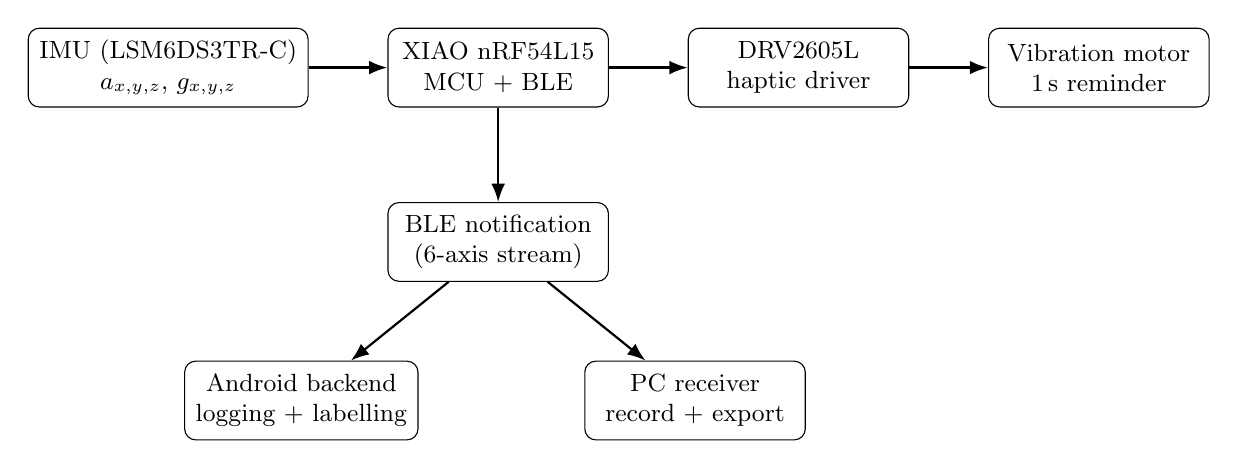
\begin{tikzpicture}[
        node distance=10mm,
        every node/.style={font=\small},
        block/.style={draw, rounded corners, align=center,
                      minimum height=10mm, minimum width=28mm,
                      inner xsep=4pt, inner ysep=4pt},
        arrow/.style={-Latex, thick}
    ]
        \node[block] (imu)   {IMU (LSM6DS3TR-C)\\$a_{x,y,z}$, $g_{x,y,z}$};
        \node[block, right=of imu] (mcu)   {XIAO nRF54L15\\MCU + BLE};
        \node[block, right=of mcu] (drv)   {DRV2605L\\haptic driver};
        \node[block, right=of drv] (motor) {Vibration motor\\1\,s reminder};
        \node[block, below=12mm of mcu] (ble) {BLE notification\\(6-axis stream)};
        \node[block, below=of ble, xshift=-25mm] (phone) {Android backend\\logging + labelling};
        \node[block, below=of ble, xshift=25mm]  (pc)    {PC receiver\\record + export};

        \draw[arrow] (imu)--(mcu);
        \draw[arrow] (mcu)--(drv);
        \draw[arrow] (drv)--(motor);
        \draw[arrow] (mcu)--(ble);
        \draw[arrow] (ble)--(phone);
        \draw[arrow] (ble)--(pc);
    \end{tikzpicture}
    \caption{Hardware and software route of the wearable prototype. The pelvis-mounted IMU is read by the XIAO nRF54L15, streamed over BLE to the Android or PC receiver backend, and connected electrically to a DRV2605L haptic driver and coin vibration motor.}
    \label{fig:system_architecture}
\end{figure*}

The Seeed Studio XIAO nRF54L15 Sense was used as the central hardware platform. It was selected because it integrates the microcontroller, the LSM6DS3TR-C IMU, and the BLE radio on a single compact board. This reduces wiring, board area, and component count compared with a separate microcontroller and sensor module.

The LSM6DS3TR-C IMU is the sensing element used to measure pelvis-region motion. It provides three-axis acceleration and three-axis angular velocity, which are sufficient for the binary movement-detection task studied in this thesis.

The DRV2605L was used as the haptic driver between the microcontroller and the vibration motor. It provides the actuator interface controlled by the XIAO firmware.

The vibration actuator was an 8~mm by 3~mm coin vibration motor. This motor was selected because it is small and can provide a local tactile cue at the lower back. Its rated voltage is 3--5~V, and its rated current is 67~mA.

The 500~mAh battery provided an internal power source. The 3D-printed perforated carrier plate and orange enclosure provided the housing. The XIAO nRF54L15 Sense and the DRV2605L were mounted on the black carrier plate and fixed with hot-melt glue. The battery is housed inside the enclosure, which measures \(5.4 \times 3.0 \times 1.5~\mathrm{cm}\). The wearable prototype component cost was below EUR 30 (XIAO board $\approx$EUR 15, DRV2605L module and motor below EUR 10, battery and printed enclosure together $\approx$EUR 5).

The enclosure was designed as a functional research prototype rather than a final consumer device. The printed body protects the battery and gives a flat contact surface for attachment, while the perforated carrier plate leaves the electronics visible and accessible for debugging. This choice made it easier to adjust wiring and firmware during development.

\subsubsection{Hardware Interfaces and Connections}

The hardware uses two wired interfaces in addition to the on-board IMU and BLE radio. First, the XIAO and the DRV2605L are connected through power and an \(I^2C\) bus. The XIAO ground (GND) and 3V3 supply pins are connected to the DRV2605L GND and VIN pins. XIAO pin D4 serves as the serial data line (SDA), and XIAO pin D5 serves as the serial clock line (SCL). Second, the vibration motor is connected to the positive and negative motor output terminals of the DRV2605L. The connections are summarised in Table~\ref{tab:electrical_connections}. The wiring was intentionally kept minimal: the IMU and BLE radio are already integrated on the XIAO board, so the external circuit only adds the haptic driver, motor, and battery.

\begin{table}[!htbp]
    \centering
    \footnotesize
    \caption{Electrical connections.}
    \label{tab:electrical_connections}
    \begin{tabular*}{\linewidth}{@{\extracolsep{\fill}}lll@{}}
        \toprule
        XIAO pin & DRV2605L pin & Function \\
        \midrule
        GND & GND & Common ground \\
        3V3 & VIN & Driver power supply \\
        D4 & SDA & \(I^2C\) data \\
        D5 & SCL & \(I^2C\) clock \\
        No direct XIAO pin & OUT+ / OUT- & Motor output \\
        \bottomrule
    \end{tabular*}
\end{table}

For body attachment, the enclosure is fixed to a sterile island dressing (10~cm by 15~cm) using double-sided tape, and the dressing is applied to the skin close to the sacrum, at the lower-back/pelvic region. This placement is more directly informative for lower-trunk and pelvic motion than wrist placements, and is consistent with the sacral/pelvic placement reported by Liao et al. for IMU-based pelvic-rotation detection. The placement also keeps the device near the vibration target, so the same body location is used for sensing and feedback.

\subsubsection{IMU Data and Sampling Frequency}

The firmware sampled the IMU at 208~Hz. Each sample contained six raw motion channels: three-axis acceleration \((a_x, a_y, a_z)\) and three-axis angular velocity \((g_x, g_y, g_z)\). In the firmware, acceleration is read in \si{\meter\per\second\squared} and angular velocity in radians per second from the Zephyr sensor API before being encoded for BLE transmission.

\subsubsection{BLE Output Signal and Settings}

The device exposes the IMU stream through BLE notifications. The BLE settings used by the receiver backends are listed in Table~\ref{tab:ble_identifiers}. The advertised name allows the Android and PC software to identify the wearable, the service UUID identifies the custom BLE service, and the notification UUID identifies the characteristic that emits the IMU packets.

\begin{table}[!htbp]
    \centering
    \scriptsize
    \caption{BLE advertising name and subscription identifiers.}
    \label{tab:ble_identifiers}
    \begin{tabularx}{\linewidth}{@{}l>{\raggedright\arraybackslash}X@{}}
        \toprule
        Item & Value \\
        \midrule
        Advertised name & \path{ble-imu-sensor} \\
        Service UUID & \path{12345678-1234-5678-1234-56789abcdef0} \\
        Notification UUID & \path{12345678-1234-5678-1234-56789abcdef1} \\
        \bottomrule
    \end{tabularx}
\end{table}

Each BLE notification carries a compact 12-byte payload, decoded as six little-endian signed 16-bit integers for three-axis acceleration and angular velocity (Table~\ref{tab:ble_payload_format}). The payload contains only the six motion values and leaves timestamping to the receiving software during logging.

\begin{table}[!htbp]
    \centering
    \footnotesize
    \caption{BLE notification payload format.}
    \label{tab:ble_payload_format}
    \begin{tabularx}{\linewidth}{llX}
        \toprule
        Bytes & Field & Description \\
        \midrule
        0--1   & \texttt{accel\_x} & Raw acceleration $X$ \\
        2--3   & \texttt{accel\_y} & Raw acceleration $Y$ \\
        4--5   & \texttt{accel\_z} & Raw acceleration $Z$ \\
        6--7   & \texttt{gyro\_x}  & Raw angular velocity $X$ \\
        8--9   & \texttt{gyro\_y}  & Raw angular velocity $Y$ \\
        10--11 & \texttt{gyro\_z}  & Raw angular velocity $Z$ \\
        \bottomrule
    \end{tabularx}
\end{table}

Acceleration is encoded in \(10^{-3}\,\si{\meter\per\second\squared}\) units, and angular velocity is encoded in milliradians per second.

\subsection{Android Backend}\label{sec:android_app}

The Android backend is the mobile field-collection software. The evaluated application used package \path{com.l1172.bleimuandroid}, versionName \texttt{1.0.1}, versionCode \texttt{2}, compile SDK 34, and target SDK 34. Its role was to scan for the wearable, connect to it through BLE, subscribe to the IMU notification characteristic, decode the 12-byte motion packets, and save the converted IMU values to CSV files.

The Android backend can maintain two wearable connections simultaneously, which was required for multi-device field sessions. During recording, the backend writes packets to a comma-separated values (CSV) file in the phone's external documents directory. A foreground service keeps BLE and Global Positioning System (GPS) collection active when the screen is locked. GPS samples are obtained from Android's fused location provider; each IMU row is stamped with \texttt{gps\_age\_ms}, the time difference between the IMU packet and the most recent GPS fix.

The backend stores annotation state separately for each connected wearable. When an annotation state is active, the current label is written into every CSV row received from that device until the annotation is stopped. Default labels are loaded from the app configuration, so the recording protocol can include labels such as static sitting, pelvic rotation, walking, or transport segments. Each annotation is assigned a segment identifier and a start timestamp, allowing later processing to recover labelled time segments instead of treating each row as an isolated sample.

This annotation design is important for the field protocol. The labels are not inferred automatically by the phone; they are entered during the session and later used to select clean seated segments. Recording the label on every row makes the files easy to process, while the segment identifier preserves the fact that consecutive rows belong to the same instructed activity period. Rows outside an active annotation can be kept in the raw log for completeness but excluded from the labelled analysis dataset.

The Android CSV stores one row per packet, with device identity, phone receive timestamp, six converted IMU channels, GPS metadata, and annotation fields (Table~\ref{tab:android_csv_format}). Rows without an active annotation leave the annotation columns blank.

\begin{table}[!htbp]
    \centering
    \footnotesize
    \caption{CSV fields recorded by the Android application.}
    \label{tab:android_csv_format}
    \begin{tabularx}{\linewidth}{lX}
        \toprule
        Field group & Columns \\
        \midrule
        Device + time & \texttt{device\_label}, \texttt{timestamp}, \texttt{epoch\_ms} \\
        IMU values    & \texttt{accel\_\{x,y,z\}}, \texttt{gyro\_\{x,y,z\}} \\
        GPS time      & \texttt{gps\_fix\_timestamp}, \texttt{gps\_fix\_epoch\_ms} \\
        GPS position  & \texttt{gps\_lat}, \texttt{gps\_lon} \\
        GPS quality   & \texttt{gps\_accuracy\_m}, \texttt{gps\_provider}, \texttt{gps\_age\_ms} \\
        GPS motion    & \texttt{gps\_altitude\_m}, \texttt{gps\_speed\_mps}, \texttt{gps\_bearing\_deg} \\
        Annotation    & \texttt{annotation\_label}, \texttt{annotation\_segment\_id}, \texttt{annotation\_started\_timestamp}, \texttt{annotation\_started\_epoch\_ms} \\
        \bottomrule
    \end{tabularx}
\end{table}

Before the pilot tests, the Android backend was checked for BLE scanning, per-device connection, packet logging, GPS metadata storage, and row-level annotation fields. These checks confirmed that the mobile backend could collect labelled field data from the wearable.

\subsection{PC Receiver Backend}\label{sec:pc_receiver}

The PC receiver backend is the researcher-side software for bench testing, debugging, and export. It is implemented in Python using \texttt{bleak} (\(\ge 0.20.0\)) for BLE communication and \texttt{openpyxl} (\(\ge 3.0.0\)) for Excel export. Like the Android backend, it connects to the wearable over BLE, subscribes to the notification characteristic listed in Table~\ref{tab:ble_identifiers}, and decodes the same 12-byte notification payload according to Table~\ref{tab:ble_payload_format}.

Additional derived channels, including gravity-removed motion acceleration and quaternion estimates, are computed in the receiver pipeline for later analysis.

To keep acquisition independent of display refresh or file I/O timing, incoming packets are pushed onto a queue and written to CSV by a dedicated writer thread. The receiver can also export buffered data to an Excel file using \texttt{openpyxl}. The PC backend was mainly used to verify whether the prototype produced stable decoded streams before and after field sessions.

The PC receiver writes its own CSV file with raw and derived signals (Table~\ref{tab:pc_csv_format}). Compared with the Android log, it omits annotation and GPS fields but adds gravity-removed motion acceleration and quaternion estimates.

\begin{table}[!htbp]
    \centering
    \footnotesize
    \caption{CSV fields recorded by the PC receiver.}
    \label{tab:pc_csv_format}
    \begin{tabularx}{\linewidth}{lX}
        \toprule
        Field group & Columns \\
        \midrule
        Time              & \texttt{timestamp} \\
        Raw acceleration  & \texttt{accel\_\{x,y,z\}} \\
        Motion accel.     & \texttt{accel\_motion\_\{x,y,z\}} \\
        Angular velocity  & \texttt{gyro\_\{x,y,z\}} \\
        Quaternion        & \texttt{quat\_\{w,x,y,z\}} \\
        \bottomrule
    \end{tabularx}
\end{table}

\FloatBarrier

\chapter{Implementation}\label{ch:implementation}

This chapter describes the supporting software platform used to acquire labelled IMU data and the embedded classifier implementation that runs on the XIAO nRF54L15 Sense. The implementation was designed around one data pipeline: the wearable samples the IMU, transmits the same six-channel stream to the acquisition tools during experiments, and later runs a reduced version of the trained detector on-device. Keeping the packet format shared across tools reduces the chance that bench testing, field collection, and embedded deployment describe different signals. The evaluation protocol and results are separated into Chapters~\ref{ch:evaluation} and~\ref{ch:results}.

Two acquisition tools were developed for different stages of the same workflow (Table~\ref{tab:software_roles}): an Android application for mobile field collection, and a PC receiver for bench tests, debugging, and visualisation.

For reproducibility, the Android application evaluated in this thesis is package \texttt{com.l1172.bleimuandroid}, versionName \texttt{1.0.1}, versionCode \texttt{2}, built with compile SDK 34 and target SDK 34. The PC receiver is the Python BLE receiver using \texttt{bleak} \(\ge 0.20.0\), PyQt5 \(\ge 5.15.0\), PyQtChart \(\ge 5.15.0\), and \texttt{openpyxl} \(\ge 3.0.0\). The deployable haptic firmware is the Zephyr/PlatformIO XIAO nRF54L15 build with the main thread stack set to 4{,}096 bytes.

\begin{table}[H]
    \centering
    \footnotesize
    \caption{Roles of the two data-collection tools.}
    \label{tab:software_roles}
    \begin{tabularx}{\linewidth}{lX}
        \toprule
        Tool & Main role \\
        \midrule
        Android app & Mobile field collection, two-device BLE connection, real-time packet monitoring, GPS recording, per-device activity labelling \\
        PC receiver & Researcher-side BLE connection, live visualisation, signal inspection, CSV recording, Excel export \\
        \bottomrule
    \end{tabularx}
\end{table}

\section{BLE Data Interface}\label{sec:ble_data_interface}

Both the Android application and the PC tool use the same BLE interface. The wearable advertises as \texttt{ble-imu-sensor}; the receiver subscribes to service UUID \texttt{12345678-1234-5678-1234-56789abcdef0} and notification characteristic UUID \texttt{12345678-1234-5678-1234-56789abcdef1}. Each notification carries a 12-byte payload, decoded as six little-endian signed 16-bit integers for three-axis acceleration and angular velocity (Table~\ref{tab:ble_payload_format}). In the BLE streaming firmware, acceleration is encoded in \(10^{-3}\,\si{\meter\per\second\squared}\) units and angular velocity is encoded in milliradians per second. Both receivers therefore divide acceleration by 1000 to obtain \si{\meter\per\second\squared}, and multiply gyroscope values by \(180/(\pi\cdot 10^3) \approx 0.0573\) to obtain \si{\degree\per\second}.

The payload is intentionally compact. A 12-byte notification contains only the six motion values and leaves timestamping to the receiving device during logging. This keeps wireless transmission simple and avoids a larger packet format while still preserving all channels needed for the classifier. During embedded inference, the firmware reads acceleration in \si{\meter\per\second\squared} and angular velocity in radians per second from the Zephyr sensor API, then converts angular velocity to \si{\degree\per\second} before feature extraction so that the deployed model follows the same unit convention as the logged training data.

\begin{table}[H]
    \centering
    \footnotesize
    \caption{BLE notification payload format.}
    \label{tab:ble_payload_format}
    \begin{tabularx}{\linewidth}{llX}
        \toprule
        Bytes & Field & Description \\
        \midrule
        0--1   & \texttt{accel\_x} & Raw acceleration $X$ \\
        2--3   & \texttt{accel\_y} & Raw acceleration $Y$ \\
        4--5   & \texttt{accel\_z} & Raw acceleration $Z$ \\
        6--7   & \texttt{gyro\_x}  & Raw angular velocity $X$ \\
        8--9   & \texttt{gyro\_y}  & Raw angular velocity $Y$ \\
        10--11 & \texttt{gyro\_z}  & Raw angular velocity $Z$ \\
        \bottomrule
    \end{tabularx}
\end{table}

\section{Android Field Collection}\label{sec:android_app}

The Android application scans for nearby wearable devices, connects over BLE, subscribes to the IMU notification characteristic, and records the latest acceleration and gyroscope values for each connected device. It can connect to two wearables simultaneously, which was useful for multi-device field sessions. During recording, the application writes packets to a comma-separated values (CSV) file in the phone's external documents directory. A foreground service keeps BLE and Global Positioning System (GPS) collection active when the screen is locked. GPS samples are obtained from Android's fused location provider; each IMU row is stamped with \texttt{gps\_age\_ms}, the time difference between the IMU packet and the most recent GPS fix.

The application supports per-device activity annotation. When recording is active, each connected wearable has its own label controls; the selected label is written into every CSV row received from that device until the label is stopped. Default labels are configurable, so the researcher can match the protocol (for example, static sitting, pelvic rotation, walking, or transport segments). Each annotation is assigned a segment identifier and a start timestamp, allowing later processing to recover labelled time segments instead of treating each row as an isolated sample.

This annotation design is important for the field protocol. The labels are not inferred automatically by the phone; they are entered during the session and later used to select clean seated segments. Recording the label on every row makes the files easy to process, while the segment identifier preserves the fact that consecutive rows belong to the same instructed activity period. Rows outside an active annotation can be kept in the raw log for completeness but excluded from the classifier dataset.

\begin{figure*}[!t]
    \centering
    \begin{minipage}[t]{0.31\textwidth}
        \centering
        \vspace{0pt}
        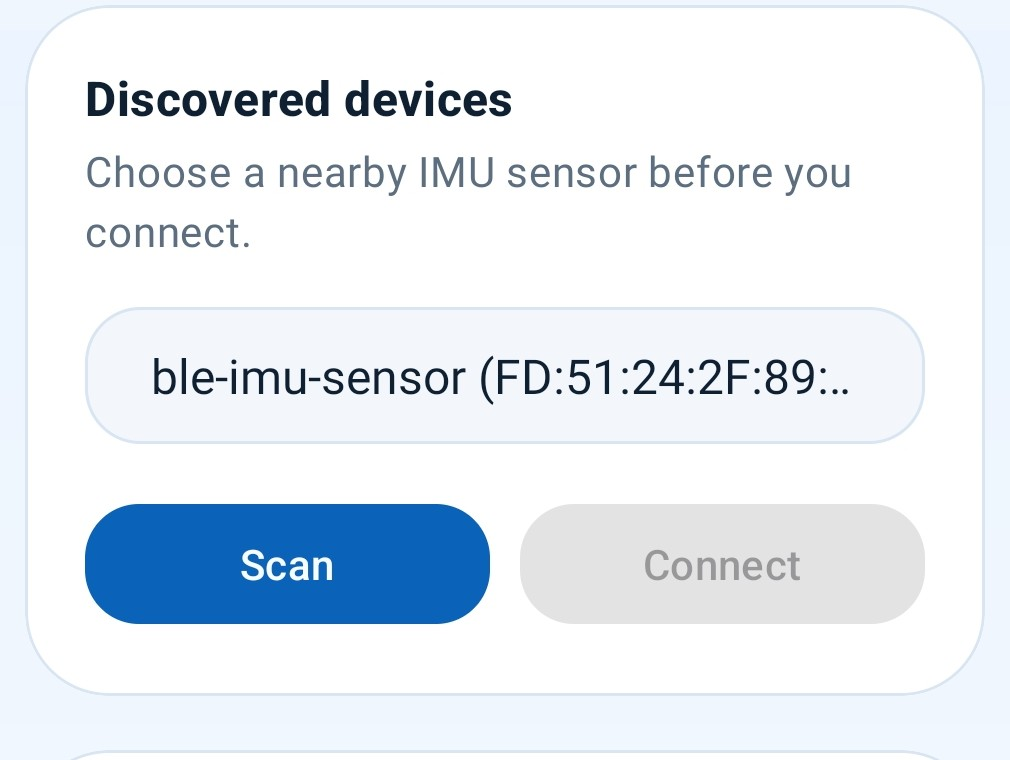
\includegraphics[width=\linewidth,height=0.28\textheight,keepaspectratio]{c4_mobile_discovery.jpg}\\
        \small (a) Device discovery and BLE connection
    \end{minipage}
    \hfill
    \begin{minipage}[t]{0.31\textwidth}
        \centering
        \vspace{0pt}
        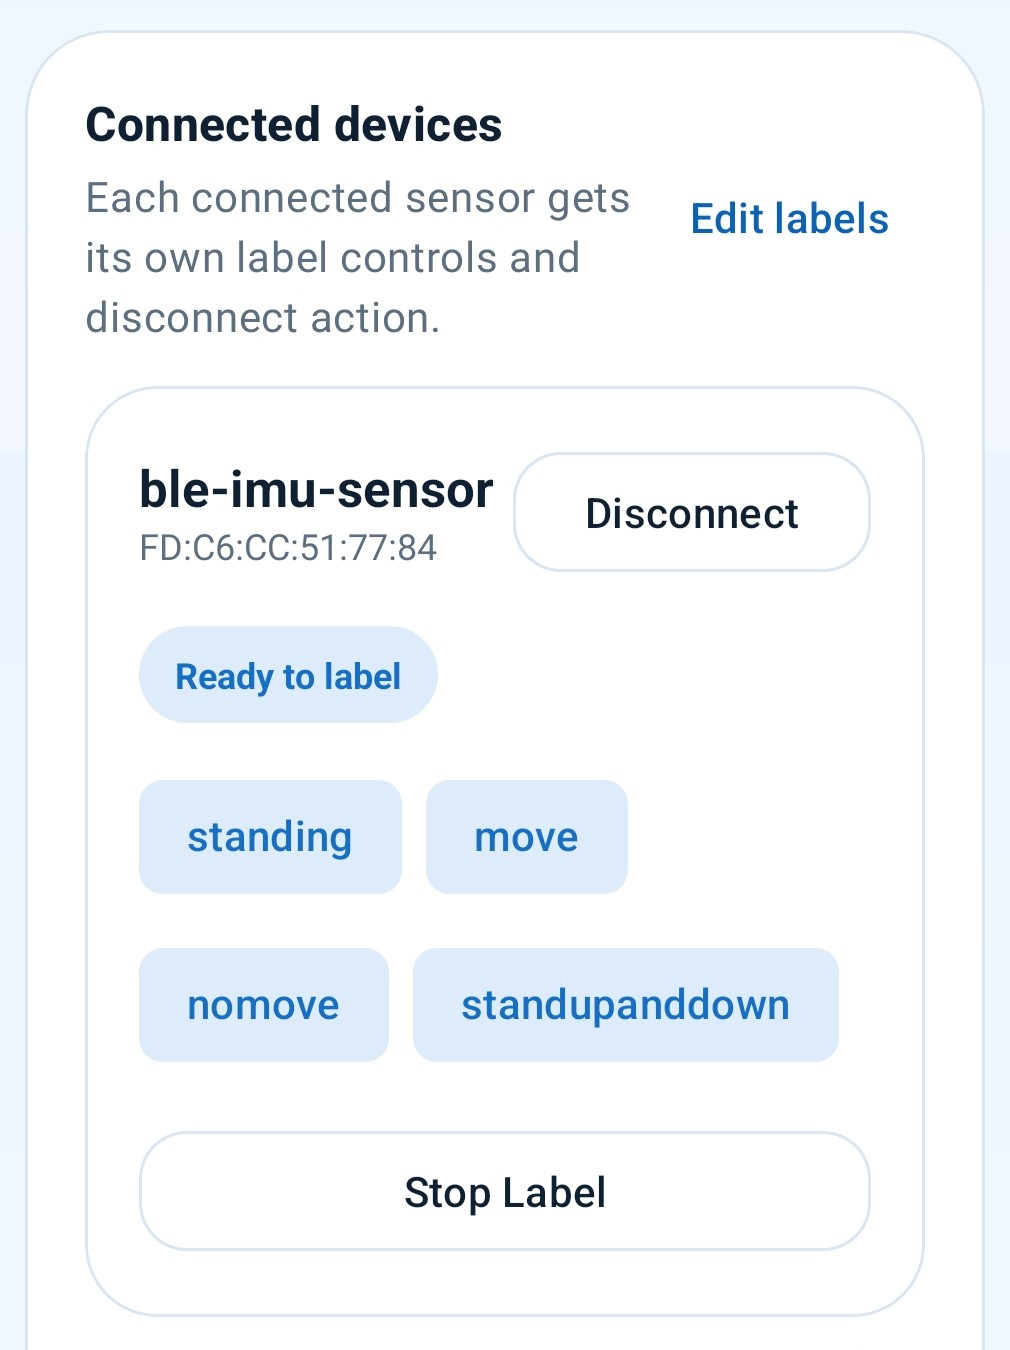
\includegraphics[width=\linewidth,height=0.28\textheight,keepaspectratio]{c4_mobile_label_controls.jpg}\\
        \small (b) Per-device activity label controls
    \end{minipage}
    \hfill
    \begin{minipage}[t]{0.31\textwidth}
        \centering
        \vspace{0pt}
        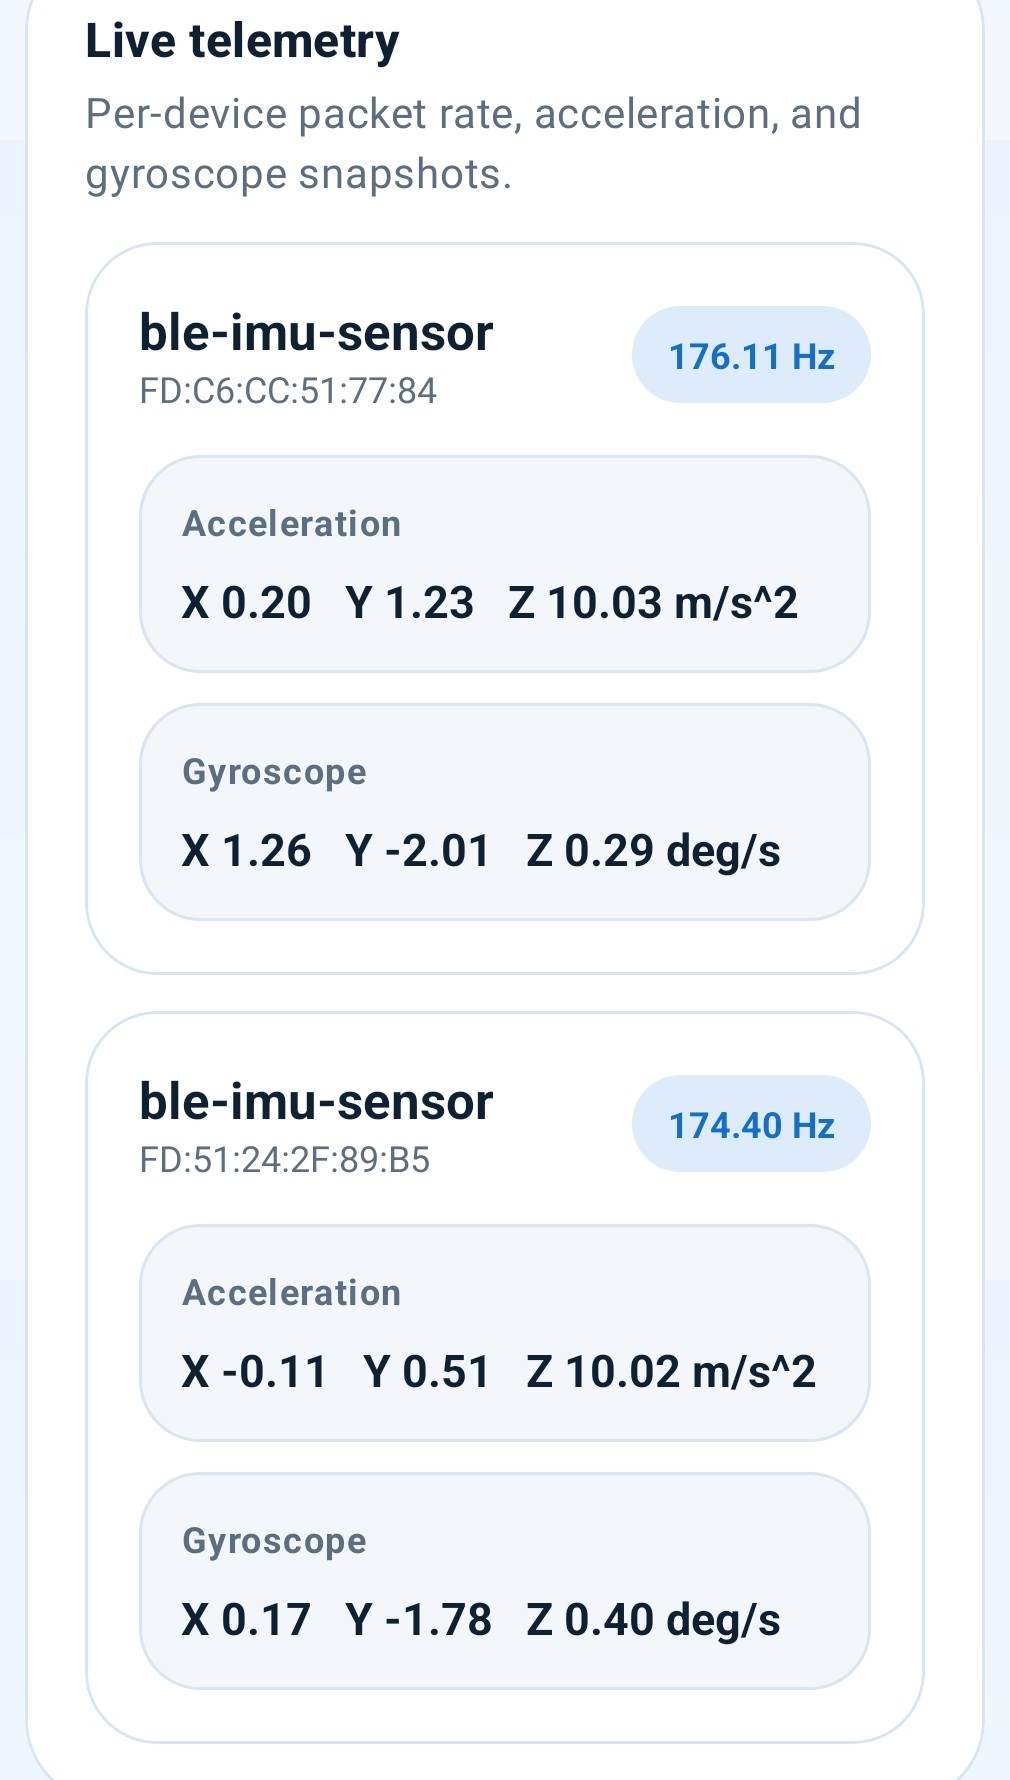
\includegraphics[width=\linewidth,height=0.28\textheight,keepaspectratio]{c4_mobile_live_telemetry_clean.jpg}\\
        \small (c) Two-device live IMU telemetry
    \end{minipage}
    \caption{Android field receiver during data collection: (a) device discovery and connection, (b) per-device activity labelling, and (c) live IMU telemetry for two connected wearable sensors.}
    \label{fig:android_app_screenshot}
\end{figure*}

The Android CSV stores one row per packet, with device identity, phone receive timestamp, six converted IMU channels, GPS metadata, and annotation fields (Table~\ref{tab:android_csv_format}). Rows without an active annotation leave the annotation columns blank.

\begin{table}[H]
    \centering
    \footnotesize
    \caption{CSV fields recorded by the Android application.}
    \label{tab:android_csv_format}
    \begin{tabularx}{\linewidth}{lX}
        \toprule
        Field group & Columns \\
        \midrule
        Device + time & \texttt{device\_label}, \texttt{timestamp}, \texttt{epoch\_ms} \\
        IMU values    & \texttt{accel\_\{x,y,z\}}, \texttt{gyro\_\{x,y,z\}} \\
        GPS time      & \texttt{gps\_fix\_timestamp}, \texttt{gps\_fix\_epoch\_ms} \\
        GPS position  & \texttt{gps\_lat}, \texttt{gps\_lon} \\
        GPS quality   & \texttt{gps\_accuracy\_m}, \texttt{gps\_provider}, \texttt{gps\_age\_ms} \\
        GPS motion    & \texttt{gps\_altitude\_m}, \texttt{gps\_speed\_mps}, \texttt{gps\_bearing\_deg} \\
        Annotation    & \texttt{annotation\_label}, \texttt{annotation\_segment\_id}, \texttt{annotation\_started\_timestamp}, \texttt{annotation\_started\_epoch\_ms} \\
        \bottomrule
    \end{tabularx}
\end{table}

\section{PC Receiver and Visualisation}\label{sec:pc_receiver}

The PC receiver is implemented in Python using \texttt{bleak} for BLE and PyQt for the interface. It uses the same notification characteristic as the Android application but serves a different role: bench testing, debugging, and live signal inspection. The interface shows the latest acceleration, gravity-removed motion acceleration, angular velocity, and quaternion estimate, with real-time plots for raw acceleration, angular velocity, and motion acceleration. To avoid blocking the GUI, incoming packets are pushed onto a queue and written to CSV by a dedicated thread. The receiver can also export the buffered data to an Excel file.

The PC tool was mainly used to inspect whether the prototype responded correctly before and after field sessions. Live plots made sensor saturation, disconnected devices, and unexpected axis behaviour visible immediately. The additional derived channels in the PC log were not required for the Android field dataset, but they were useful during development because they made movement peaks easier to inspect.

\begin{figure*}[!t]
    \centering
    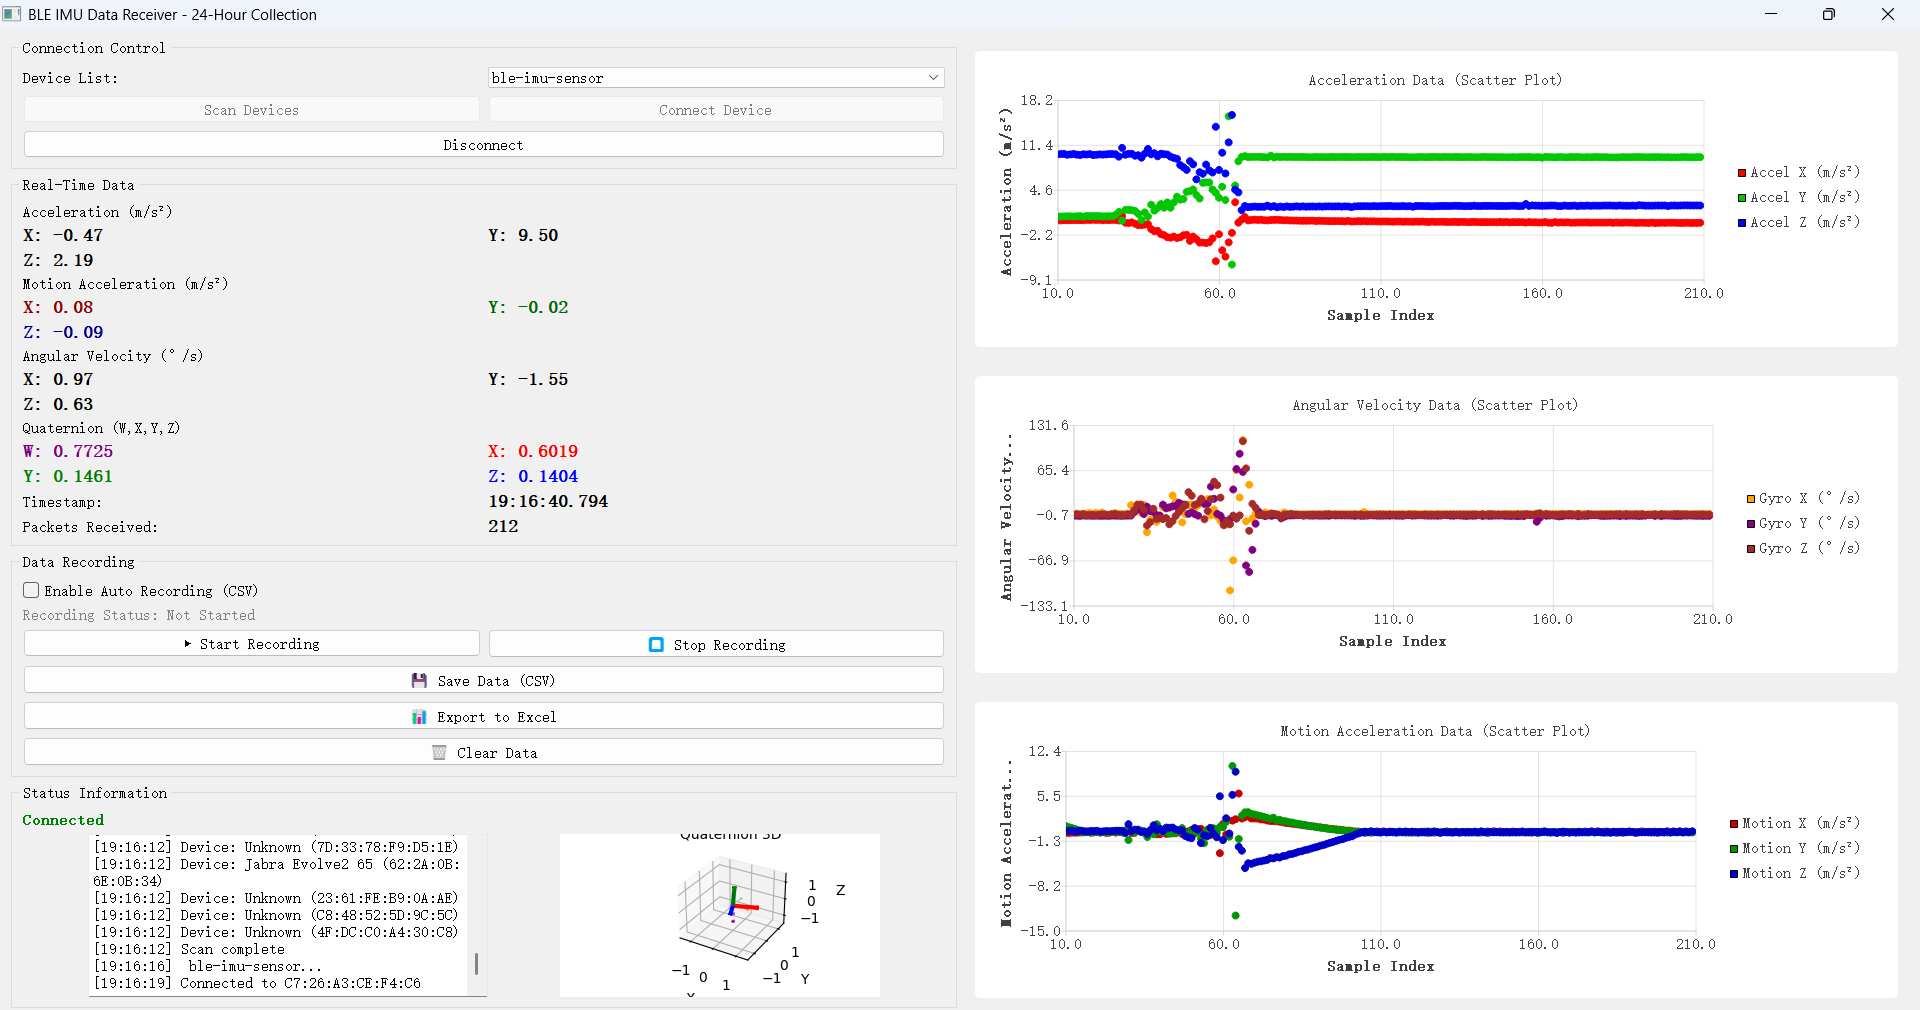
\includegraphics[width=0.92\textwidth]{c4_pc_receiver_gui.png}
    \caption{PC-based BLE receiver for researcher-side monitoring. The interface includes connection control, real-time IMU values, recording controls, status log, quaternion visualisation, and live plots for acceleration, angular velocity, and motion acceleration.}
    \label{fig:pc_receiver_gui}
\end{figure*}

The PC receiver writes its own CSV file with raw and derived signals (Table~\ref{tab:pc_csv_format}). Compared with the Android log it omits annotation and GPS fields but adds gravity-removed motion acceleration and quaternion estimates that were useful for live signal inspection during bench tests.

\begin{table}[H]
    \centering
    \footnotesize
    \caption{CSV fields recorded by the PC receiver.}
    \label{tab:pc_csv_format}
    \begin{tabularx}{\linewidth}{lX}
        \toprule
        Field group & Columns \\
        \midrule
        Time              & \texttt{timestamp} \\
        Raw acceleration  & \texttt{accel\_\{x,y,z\}} \\
        Motion accel.     & \texttt{accel\_motion\_\{x,y,z\}} \\
        Angular velocity  & \texttt{gyro\_\{x,y,z\}} \\
        Quaternion        & \texttt{quat\_\{w,x,y,z\}} \\
        \bottomrule
    \end{tabularx}
\end{table}

\section{Windowing and Feature Extraction}\label{sec:segmentation_features}

For the offline classifier, labelled seated segments are loaded from the Android CSV exports and converted into window-level feature vectors. The selection of clean field segments and the participant split are part of the evaluation method described in Chapter~\ref{ch:evaluation}. During loading, non-numeric samples are dropped, rows are sorted by epoch timestamp, and exact duplicate rows are removed.

Within each clean segment, raw IMU data are divided into sliding windows of 2~s with a 1~s step, retaining only windows with at least 50 samples. Each retained window inherits the label of its source segment. The IMU is configured at 208~Hz, but \(I^2C\) overhead and RTOS scheduling latency in the polling firmware reduce the effective read rate in clean field segments; this is handled by requiring a minimum sample count rather than assuming a fixed number of samples in every window.

The three derived signals were acceleration magnitude \(\|\mathbf{a}\|\), gravity-removed acceleration magnitude \(|\|\mathbf{a}\|-9.80665|\), and gyroscope magnitude \(\|\boldsymbol{\omega}\|\). For each of the six raw channels and these three derived magnitude signals, ten time-domain statistics were computed: mean, standard deviation, minimum, maximum, range, root-mean-square, median, interquartile range, mean absolute first difference, and standard deviation of the first difference. This yields a 90-dimensional feature vector per window.

\section{Compact KNN for Embedded Deployment}\label{sec:compact_knn}

A full KNN implementation is memory-heavy because it stores the training examples as its reference set. The deployed firmware therefore uses two reductions: a 12-feature subset (Table~\ref{tab:ch6_compact_knn_features}) and KMeans prototype compression. The feature subset is dominated by gyroscope and acceleration-range information, which matches the expected signal difference between static sitting and deliberate pelvic movement. The training and held-out evaluation procedure used to fix the final model configuration is described in Chapter~\ref{ch:evaluation}.

Before compression and inference, each selected feature is standardised using mean and standard-deviation values exported from the training pipeline. Within each labelled class on the standardised training windows, KMeans (\texttt{random\_state=42}, \texttt{n\_init=10}) extracts 64 centres, yielding 128 stored prototypes in total. Inference compares the current window against these prototypes using a distance-weighted KNN with \(k=7\). The exported firmware header contains the selected feature order, scaling values, prototype coordinates, class labels, and KNN setting.

\begin{table}[H]
    \centering
    \footnotesize
    \caption{Feature subset used by the compact prototype-based KNN. Names match the order used in the generated firmware header.}
    \label{tab:ch6_compact_knn_features}
    \begin{tabularx}{\linewidth}{lX}
        \toprule
        Signal group & Selected feature names \\
        \midrule
        Gyroscope $x$        & \texttt{gyro\_x\_rms}, \texttt{gyro\_x\_std}, \texttt{gyro\_x\_range} \\
        Gyroscope magnitude  & \texttt{gyro\_mag\_std}, \texttt{gyro\_mag\_max}, \texttt{gyro\_mag\_rms}, \texttt{gyro\_mag\_range}, \texttt{gyro\_mag\_mean} \\
        Acceleration $z$     & \texttt{accel\_z\_max}, \texttt{accel\_z\_range}, \texttt{accel\_z\_std} \\
        Accel.\ motion mag.  & \texttt{acc\_motion\_mag\_std} \\
        \bottomrule
    \end{tabularx}
\end{table}

The compact KNN model was integrated into the firmware. The device samples the IMU at a 5~ms polling interval, accumulates non-overlapping 2~s windows, computes the 12 window-level features online, and classifies each window as static sitting or pelvic rotation. This embedded cycle uses the same 2~s window duration and feature definitions as the offline analysis, but not the 1~s overlapping offline step. When pelvic rotation is detected, the inactivity timer is reset; otherwise, after 10~min without a detected pelvic-rotation window, the DRV2605L drives the vibration motor for one second. Per-window inference latency was measured on the device using the hardware cycle counter (\texttt{k\_cycle\_get\_64}). During deployment, the default Zephyr main thread stack size was too small once the \(I^2C\) driver, logging, and window processing were used together. Setting the main thread stack size to 4{,}096 bytes resolved a silent stack-overflow fault at startup.

\clearpage
% This file is intentionally retained as a placeholder after the structure
% revision. The current methods content is split across chapters/02-design.tex
% and chapters/03-implementation.tex under one "Methods" chapter.
%
% thesis.tex no longer inputs this file.

\clearpage
\chapter{Results}\label{ch:results}

This chapter reports the results from the evaluation methods in Chapter~\ref{ch:evaluation}. The results are grouped by the same evidence chain used in the thesis: sensor agreement with Shimmer, pilot field-worn trend agreement, detection performance on the labelled train-sitting dataset, and embedded timing of the compact KNN.

\section{Sensor Agreement Results}\label{sec:results_sensor_agreement}

\subsection{Co-Located Shimmer/XIAO Agreement}

Figure~\ref{fig:shimmer_xiao_comparison} shows the aligned time-series comparison for the co-located recording. The XIAO and Shimmer signals show the same main movement peaks across all acceleration and gyroscope channels. Across all axes, acceleration correlations ranged from 0.856 to 0.923 and gyroscope correlations from 0.816 to 0.864 (Table~\ref{tab:colocated_validation_results}). The estimated lag stayed between \(-0.020\) and 0~s, and NRMSE values ranged from 0.425 to 0.613.

\begin{figure*}[!tbp]
    \centering
    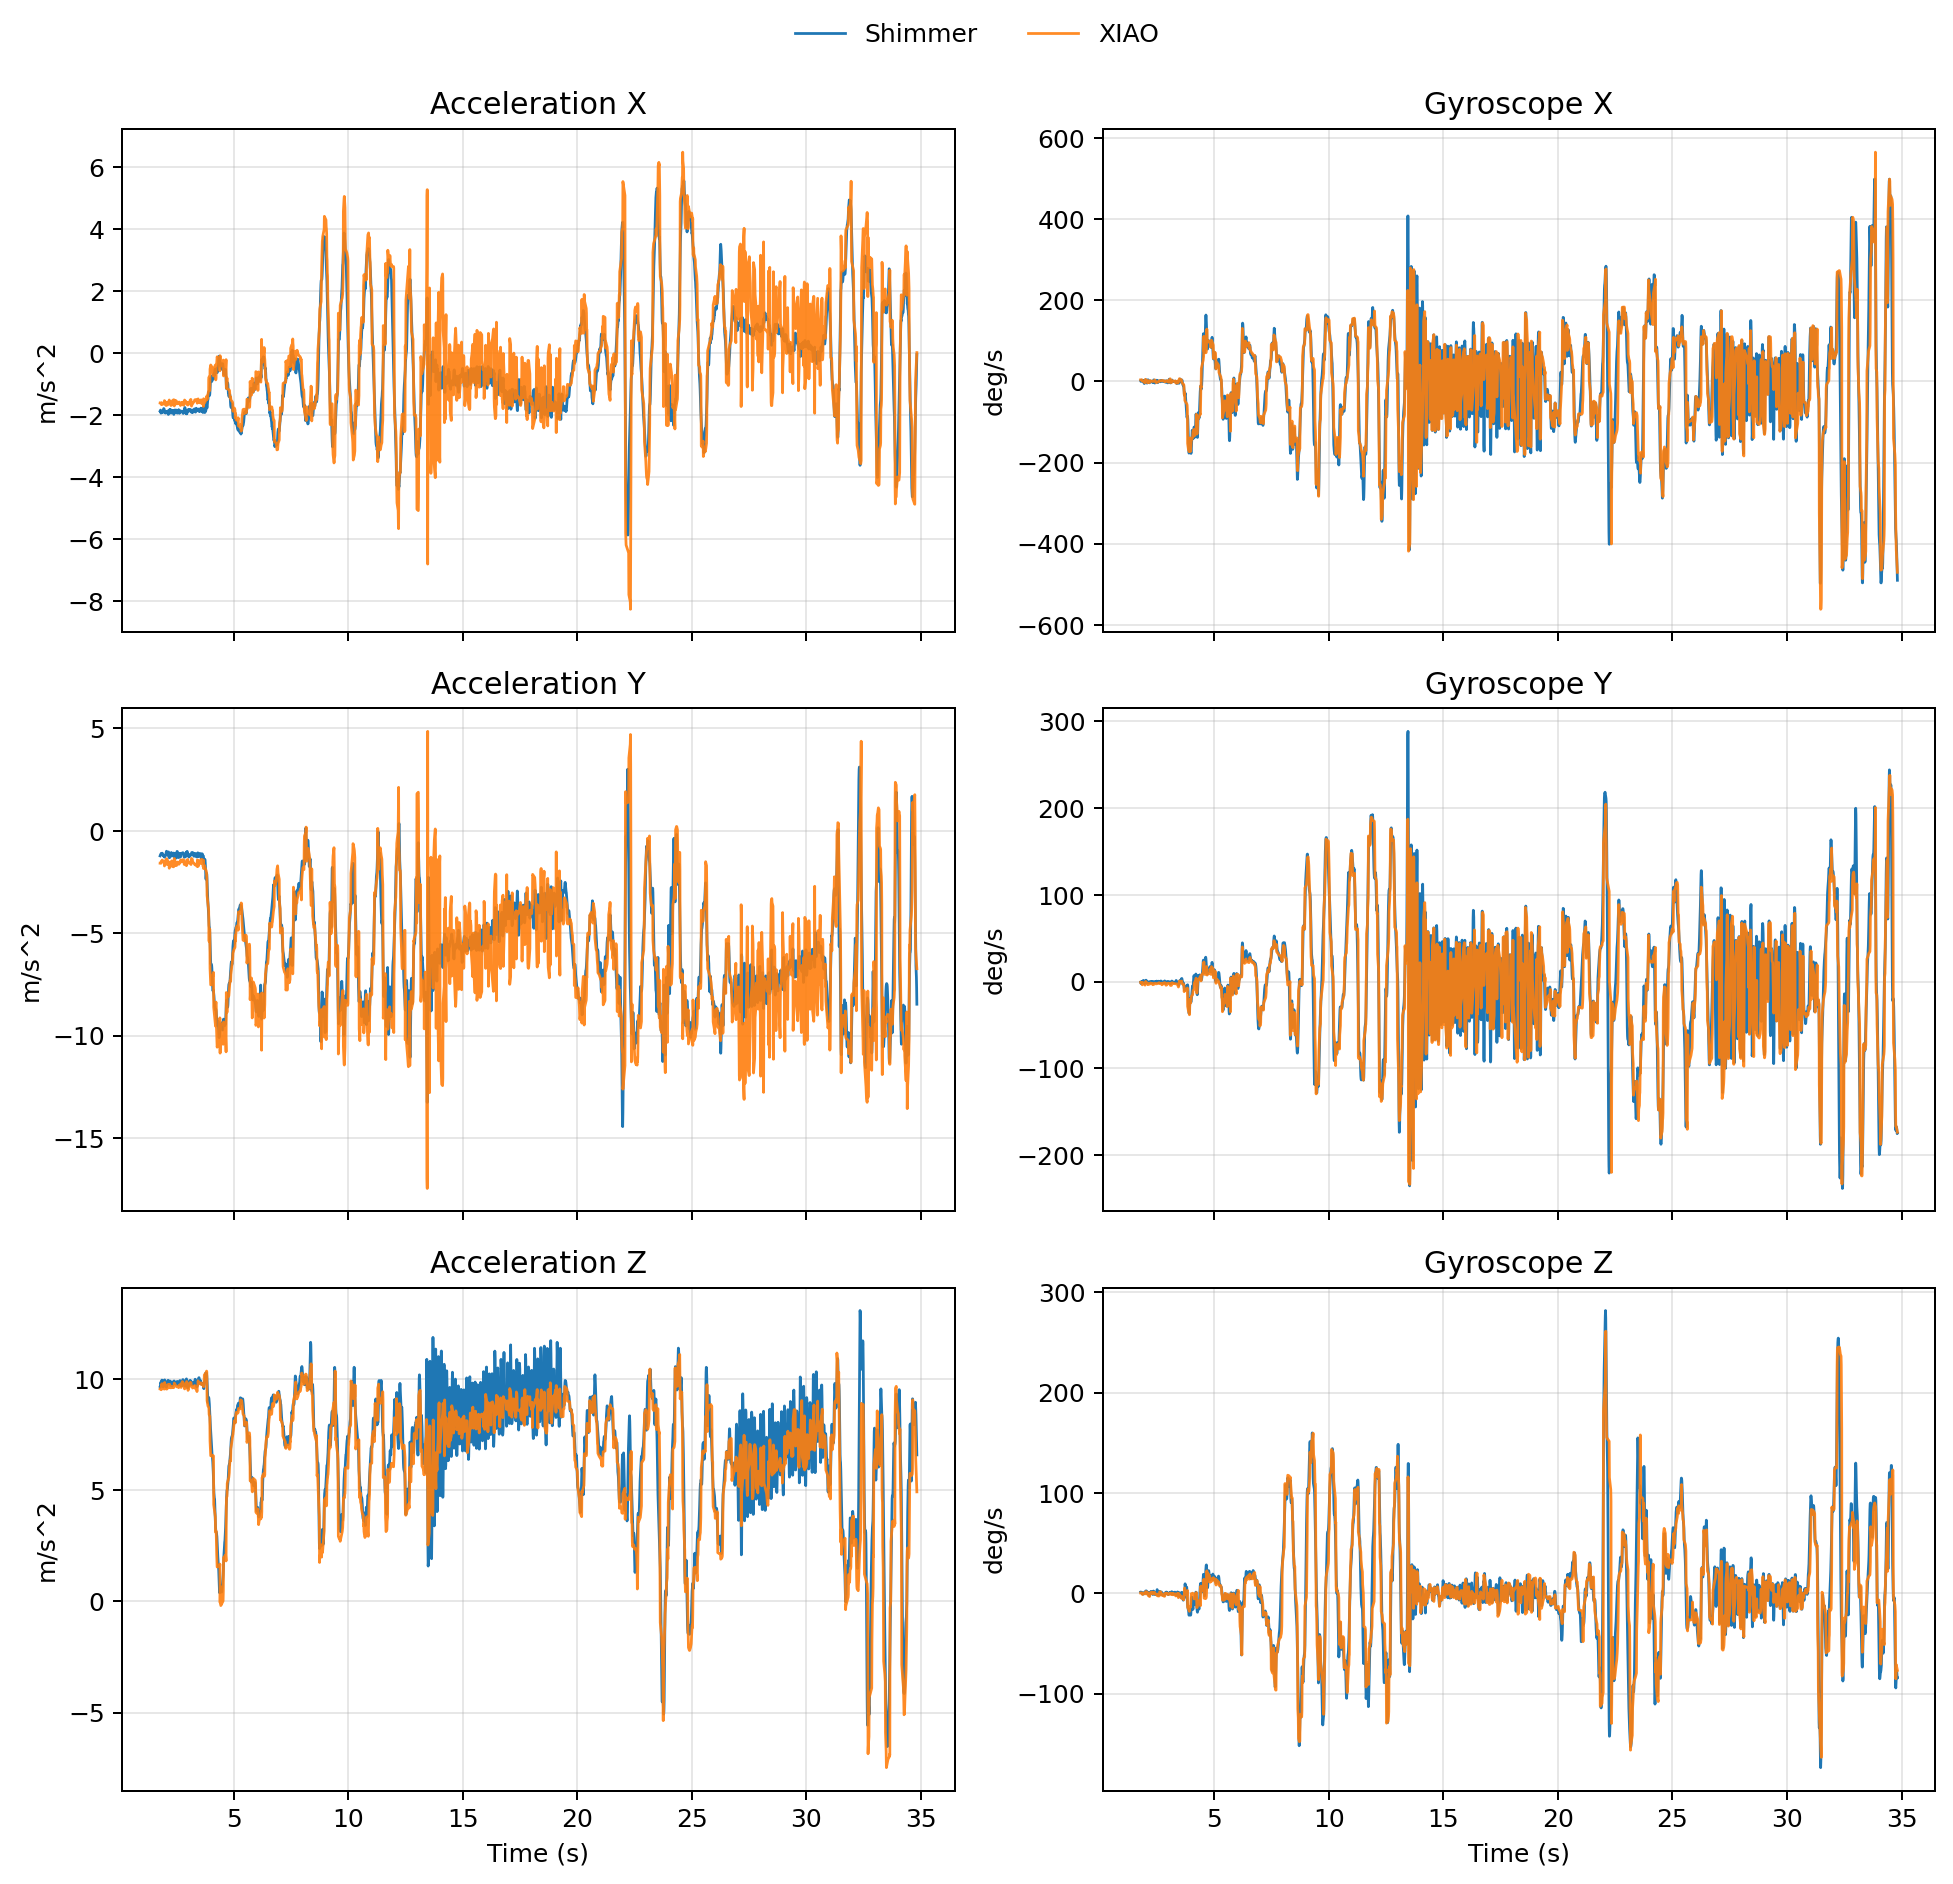
\includegraphics[width=0.94\textwidth,height=0.58\textheight,keepaspectratio]{shimmer_xiao_comparison.png}
    \caption{Aligned co-located waveform comparison between the Shimmer reference and the custom XIAO-based wearable, across the three acceleration and three gyroscope axes.}
    \label{fig:shimmer_xiao_comparison}
\end{figure*}

\begin{table}[H]
    \centering
    \scriptsize
    \caption{Co-located agreement after alignment.}
    \label{tab:colocated_validation_results}
    \begin{tabular*}{\linewidth}{@{\extracolsep{\fill}}llrrrr@{}}
        \toprule
        Signal & Axis & r & Max r & Lag (s) & NRMSE \\
        \midrule
        Accel & X & 0.907 & 0.910 & -0.010 & 0.517 \\
        Accel & Y & 0.856 & 0.856 & -0.010 & 0.613 \\
        Accel & Z & 0.923 & 0.923 & -0.010 & 0.425 \\
        Gyro  & X & 0.838 & 0.838 &  0.000 & 0.568 \\
        Gyro  & Y & 0.816 & 0.816 &  0.000 & 0.601 \\
        Gyro  & Z & 0.864 & 0.881 & -0.020 & 0.521 \\
        \bottomrule
    \end{tabular*}
\end{table}

The co-located results support the use of the XIAO signal for trend-level movement detection. The correlations indicate similar temporal patterns, while the non-zero NRMSE values show that the two sensors should not be treated as amplitude-equivalent measurement systems.

\subsection{Pilot Field-Worn Trend Agreement}

The field-worn trend comparison used the two usable paired recordings from the pilot study. Acceleration motion magnitude correlated at 0.918 for P1 and 0.855 for P2, while gyroscope magnitude correlated at 0.908 for P1 and 0.864 for P2. After lag correction, maximum cross-correlations reached 0.915--0.981. The estimated best lag was 1.2--1.3~s (Table~\ref{tab:field_trend_results}). Figure~\ref{fig:field_trend_comparison} shows the corresponding long trend comparison.

\begin{table}[H]
    \centering
    \scriptsize
    \caption{Field-worn trend agreement in the pilot study. P1 and P2 are participant identifiers.}
    \label{tab:field_trend_results}
    \begin{tabular*}{\linewidth}{@{\extracolsep{\fill}}llrrrr@{}}
        \toprule
        Part. & Signal & r & Max r & Lag (s) & NRMSE \\
        \midrule
        P1 & Accel.\ mag. & 0.918 & 0.938 & 1.20 & 0.530 \\
        P1 & Gyro mag.    & 0.908 & 0.974 & 1.20 & 0.232 \\
        P2 & Accel.\ mag. & 0.855 & 0.915 & 1.30 & 0.476 \\
        P2 & Gyro mag.    & 0.864 & 0.981 & 1.30 & 0.206 \\
        \bottomrule
    \end{tabular*}
\end{table}

\begin{figure*}[!tbp]
    \centering
    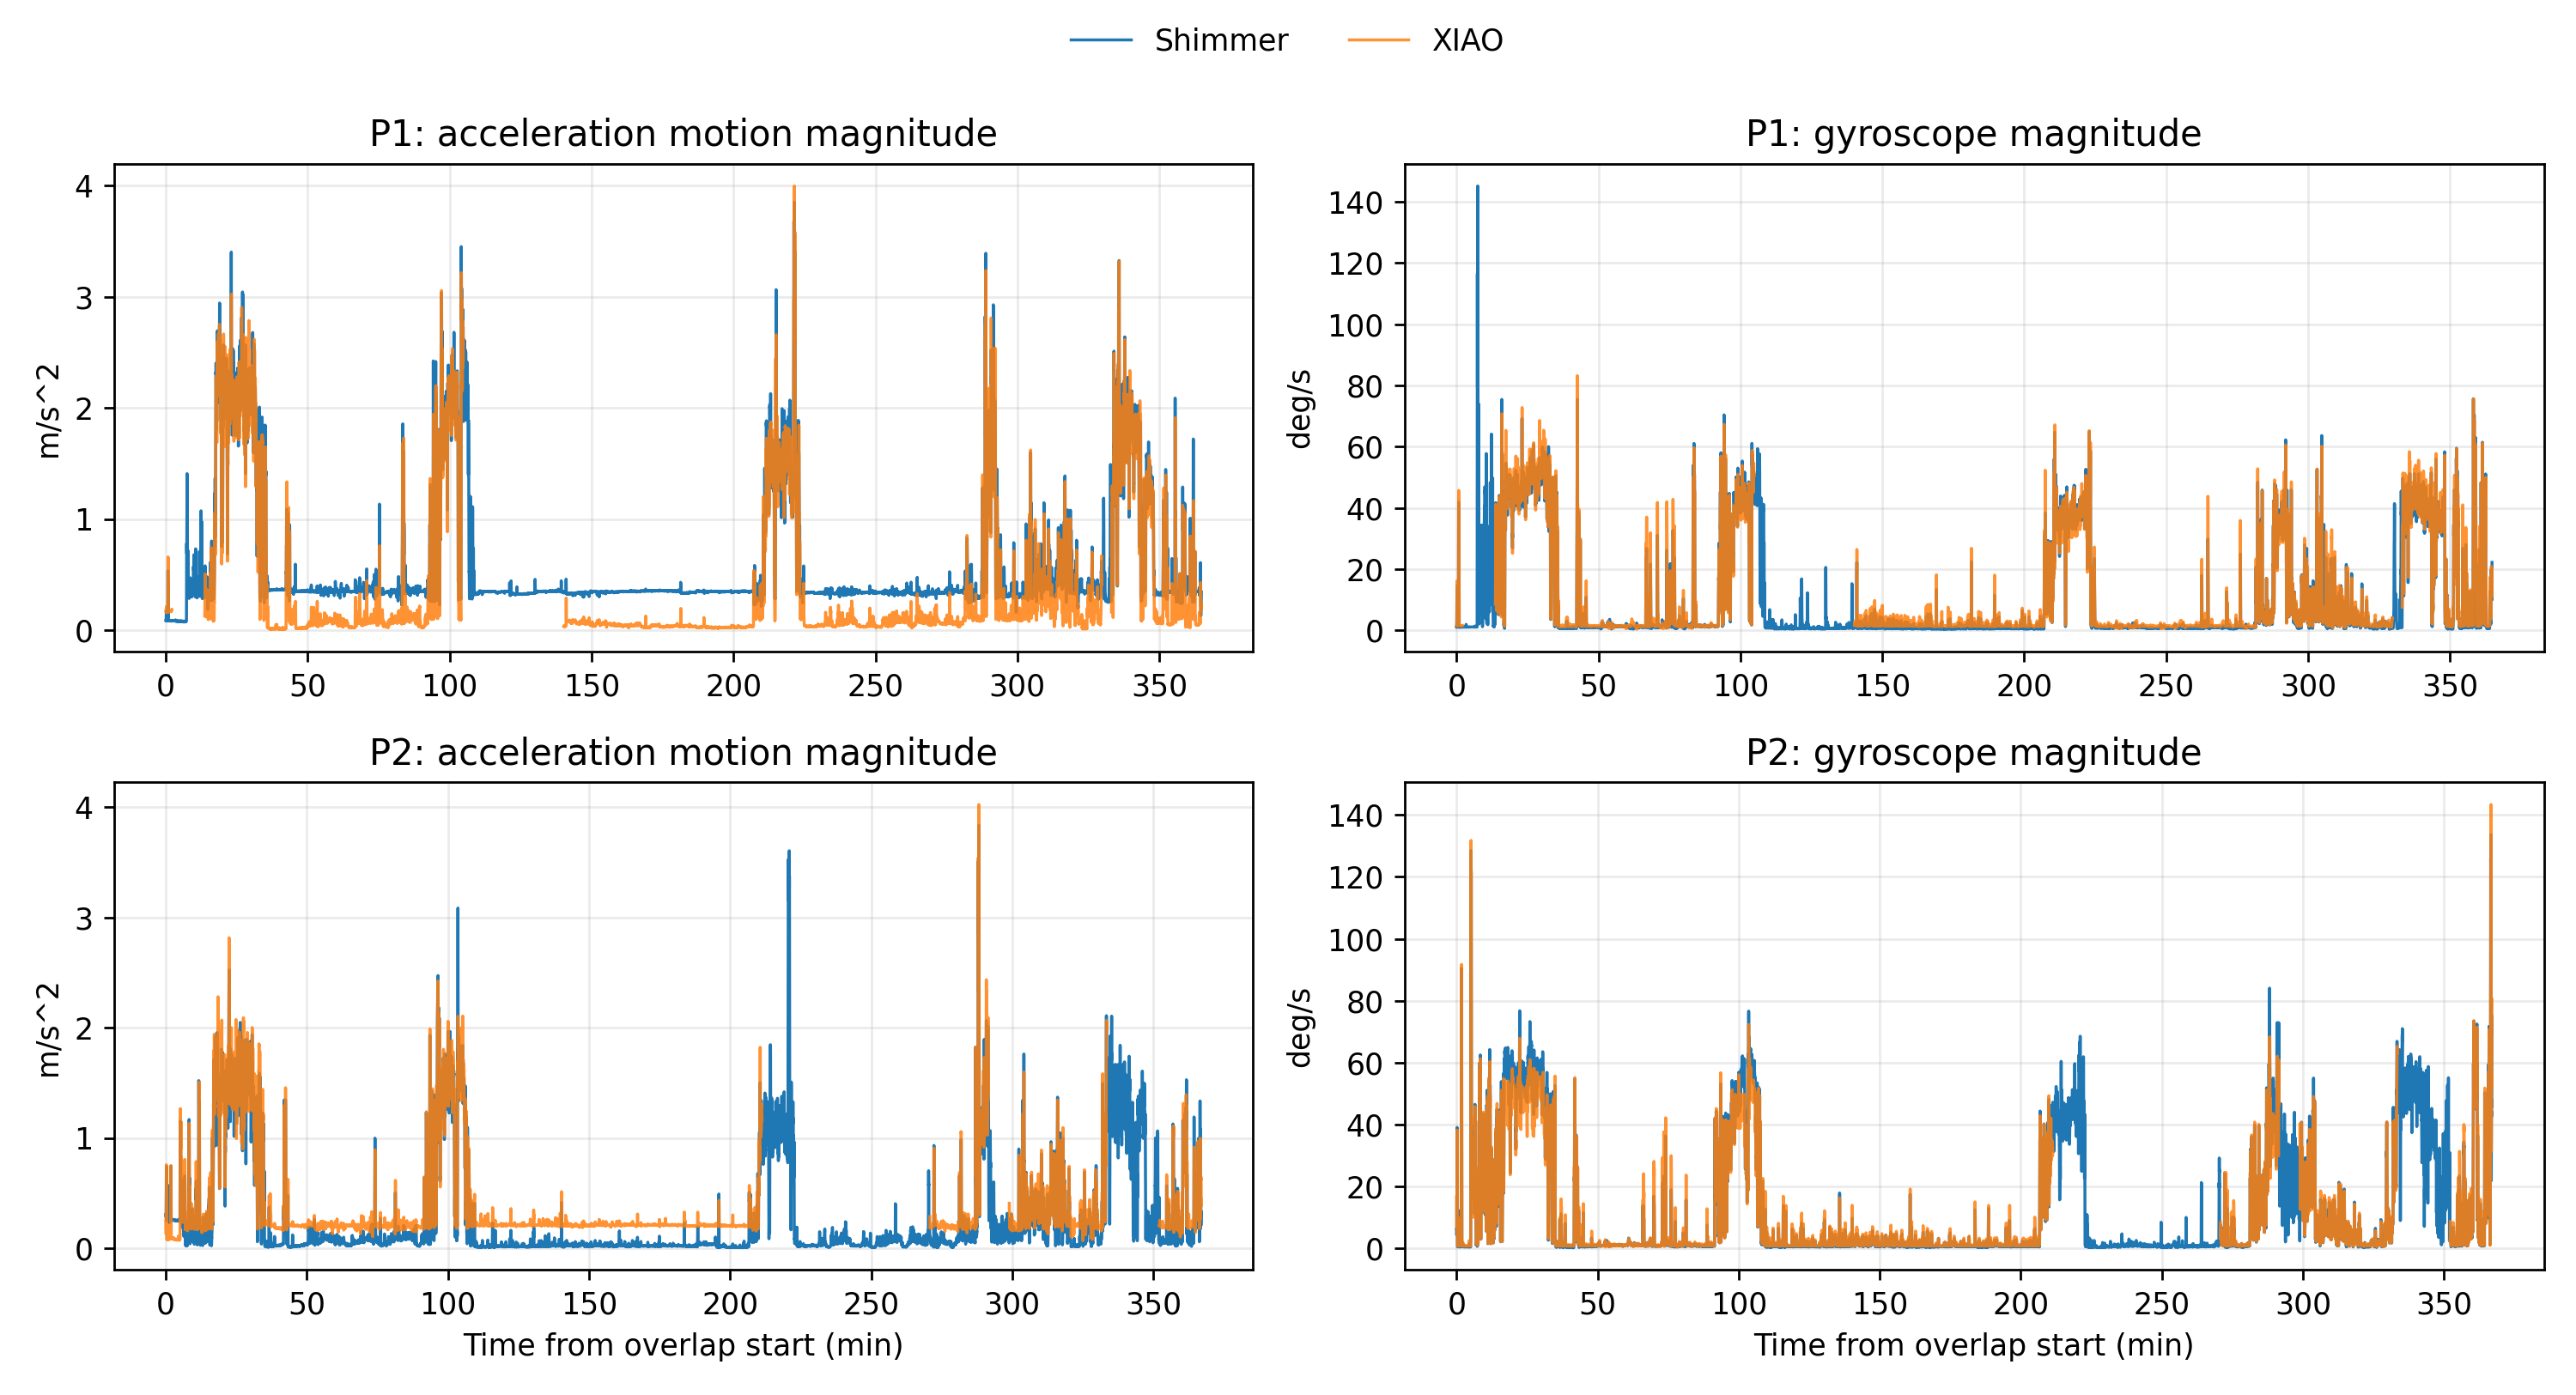
\includegraphics[width=0.94\textwidth,height=0.42\textheight,keepaspectratio]{c5_field_trend_comparison.png}
    \caption{Long field-worn trend comparison for two pilot-study participants. Signals are shown as acceleration motion magnitude and gyroscope magnitude over the overlapping recording period, after 10~Hz resampling and centred 5~s moving-average smoothing for visualisation only.}
    \label{fig:field_trend_comparison}
\end{figure*}

The field-worn correlations are lower than a controlled laboratory equivalence test would require, but that is not the claim being made here. The result shows that the XIAO captured long movement trends similar to the Shimmer reference during the pilot outing. The 1.2--1.3~s lag indicates a timing-chain offset in the field setup and is discussed in Chapter~\ref{ch:discussion}.

\section{Detection Results}\label{sec:results_detection}

\subsection{Classifier Comparison}

Table~\ref{tab:ch6_model_results} reports the held-out performance of all five classifiers on participant 5. Static sitting outnumbers pelvic rotation 21:1 in the test set, so balanced accuracy and pelvic-rotation F1-score are more informative than accuracy alone. KNN achieved the highest F1-score at 0.957.

\begin{table}[H]
    \centering
    \footnotesize
    \caption{Held-out participant-5 classification results. Precision, recall, and F1 are for the pelvic-rotation class.}
    \label{tab:ch6_model_results}
    \begin{tabular*}{\linewidth}{@{\extracolsep{\fill}}lrrrrr@{}}
        \toprule
        Model & Acc & Bal.\ acc & P & R & F1 \\
        \midrule
        LR  & 0.909 & 0.912 & 0.320 & 0.915 & 0.474 \\
        SVM & 0.964 & 0.970 & 0.557 & 0.976 & 0.709 \\
        DT  & 0.978 & 0.925 & 0.711 & 0.867 & 0.781 \\
        RF  & 0.993 & 0.921 & 0.993 & 0.842 & 0.911 \\
        KNN & 0.996 & 0.969 & 0.975 & 0.939 & 0.957 \\
        \bottomrule
    \end{tabular*}
\end{table}

Out of 165 pelvic-rotation windows, the selected KNN correctly identified 155 and missed 10. Out of 3{,}497 static-sitting windows, it classified 3{,}493 correctly and misclassified 4 as pelvic rotation. The corresponding confusion matrix is shown in Figure~\ref{fig:ch6_knn_confusion_matrix}.

\begin{figure}[!tbp]
    \centering
    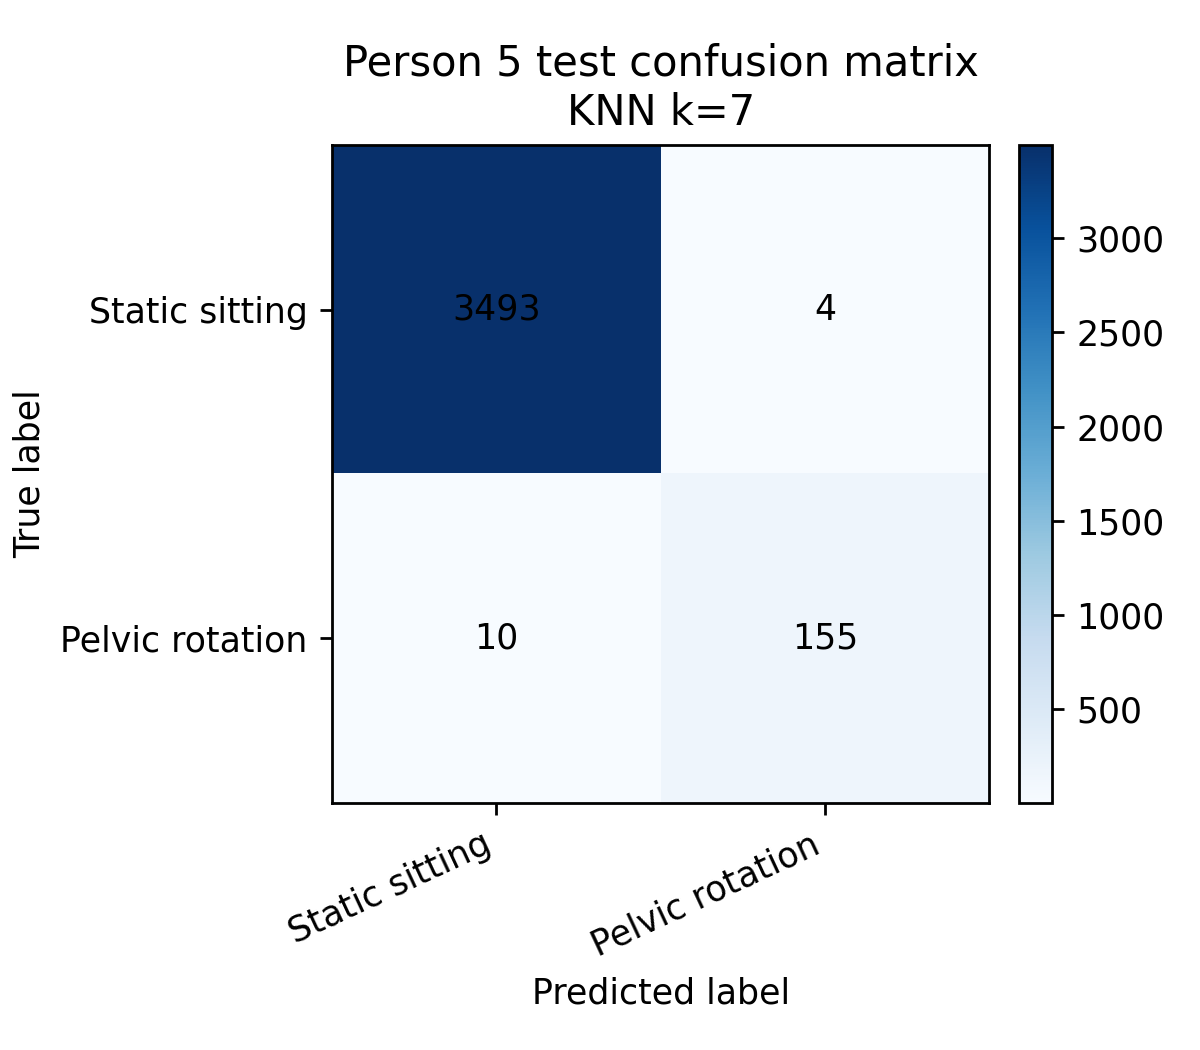
\includegraphics[width=0.76\linewidth]{ch6_person5_confusion_matrix_best_f1.png}
    \caption{Confusion matrix of the selected \(k=7\) KNN on held-out participant 5.}
    \label{fig:ch6_knn_confusion_matrix}
\end{figure}

\subsection{Compact KNN and On-Device Timing}

The compact prototype-based KNN (12 features, 128 KMeans prototypes), described in Section~\ref{sec:compact_knn}, achieved accuracy 0.996, balanced accuracy 0.963, precision 0.994, recall 0.927, and an F1-score of 0.959 on the held-out participant. The full baseline used 90 features and 9{,}391 reference windows, whereas the compact model used 12 features and 128 prototypes (Figure~\ref{fig:full_vs_compact_knn}). The compact model therefore had slightly higher precision and lower recall than the full KNN, and the comparison changes both the feature set and the reference-set size.

\begin{figure*}[!tbp]
    \centering
    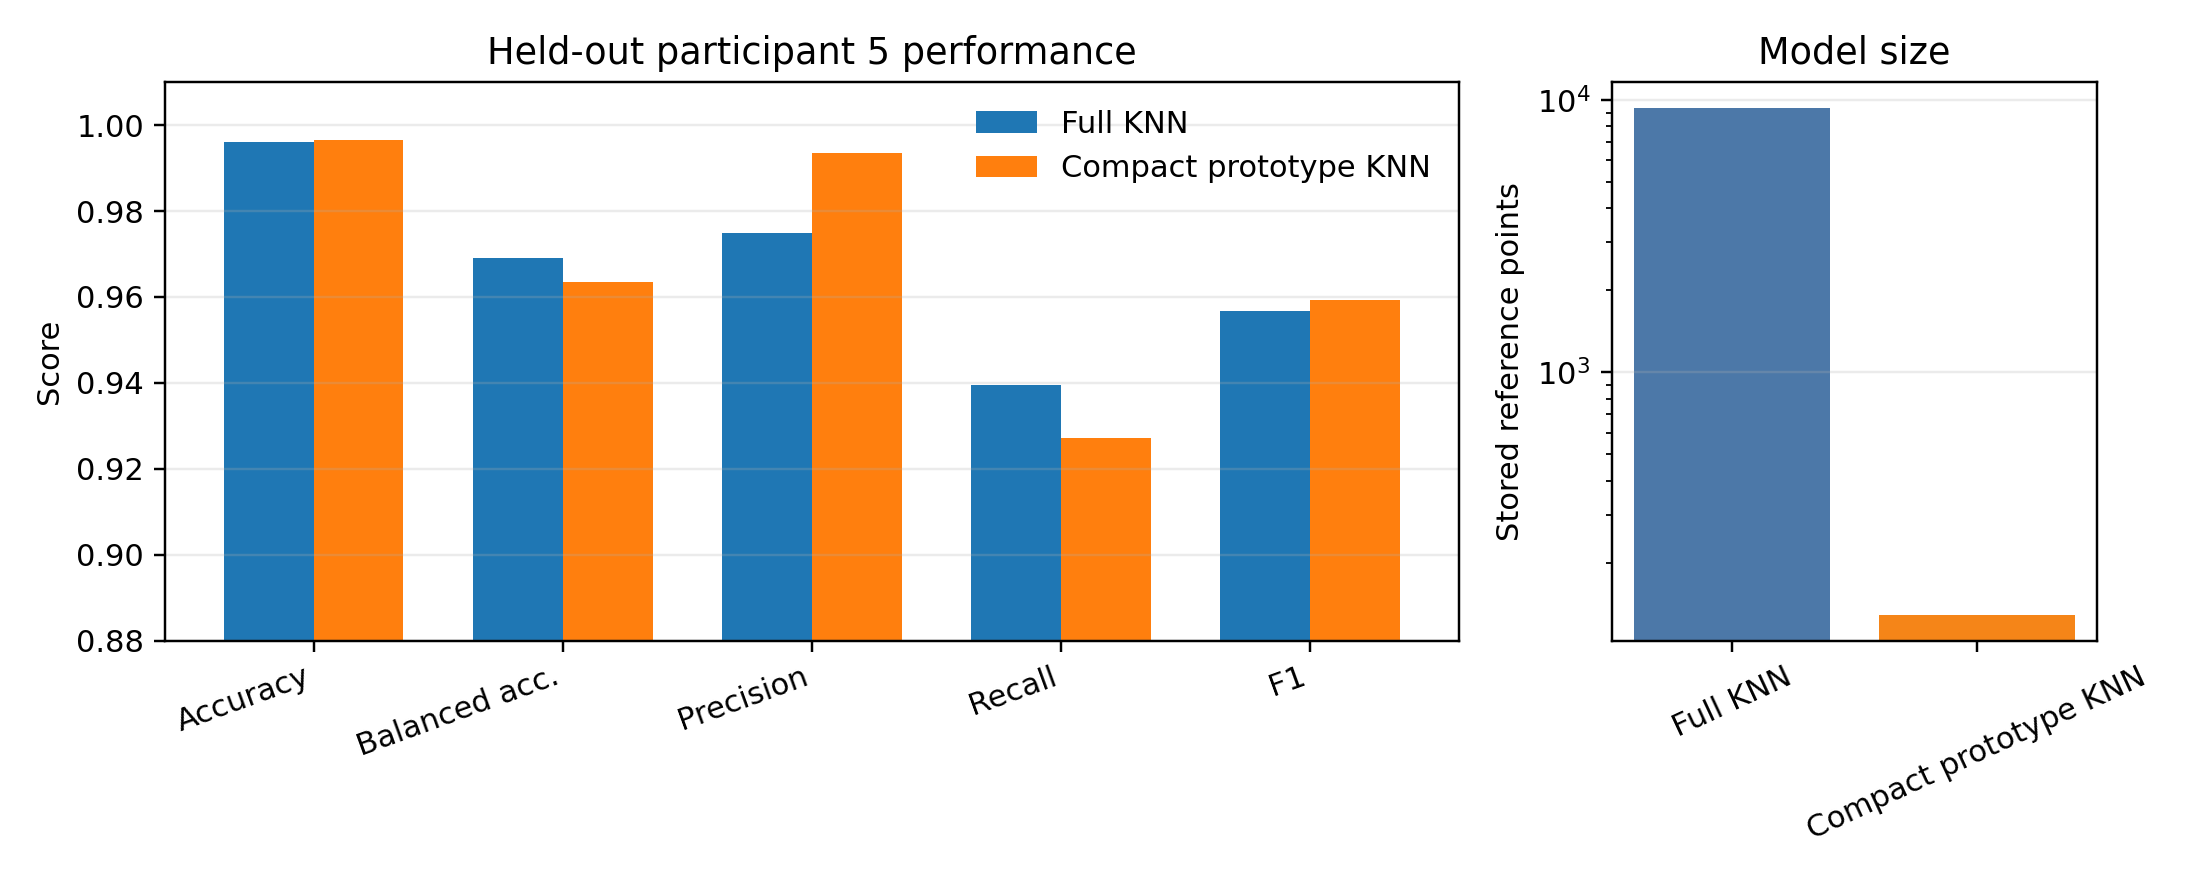
\includegraphics[width=0.92\textwidth]{ch6_full_vs_compact_knn_comparison.png}
    \caption{Comparison between the offline full KNN (90 features, 9{,}391 reference windows) and the compact prototype-based KNN (12 features, 128 KMeans prototypes) used for embedded deployment.}
    \label{fig:full_vs_compact_knn}
\end{figure*}

Table~\ref{tab:knn_timing} summarises per-window inference timing measured across 24 consecutive non-overlapping 2~s windows on the XIAO nRF54L15 Sense. The timing measurement includes the compact feature extraction path and the KNN distance computation for the stored prototypes.

\begin{table}[H]
    \centering
    \footnotesize
    \caption{On-device execution time of the compact KNN.}
    \label{tab:knn_timing}
    \begin{tabularx}{\linewidth}{lXX}
        \toprule
        Stage & Mean & Range \\
        \midrule
        KNN inference only           & 2.70~ms & 2.67--2.73~ms \\
        Features + KNN total         & 2.73~ms & 2.70--2.76~ms \\
        \bottomrule
    \end{tabularx}
\end{table}

The 2.73~ms total is below 0.15\% of the 2{,}000~ms window period. This percentage describes compute time only; it is not a power-consumption or battery-life measurement. The deployed firmware uses 56.3~KB of flash and 9.3~KB of RAM, leaving headroom within the target's available flash and RAM budget for the Zephyr RTOS, BLE stack, and future extensions.

\clearpage
\chapter{Discussion}\label{ch:discussion}

This chapter discusses the results in the same objective order used in Chapters~\ref{ch:methods} and~\ref{ch:results}. The discussion first considers the prototype as an integrated wearable platform, then the detection task, then the Shimmer/XIAO sensing evidence, and finally the embedded reminder feasibility.

\section{Objective 1: Prototype Feasibility and Engineering Trade-Offs}

The prototype addresses Objective~1 by integrating the main technical components required for a pelvis-focused reminder platform: local IMU sensing, BLE streaming, labelled Android collection, PC inspection, compact embedded classification, and local haptic actuation. This positions the work between sedentary-behaviour interventions \cite{stephenson2017technology_sedentary_meta} and wearable movement sensing \cite{papi2017wearable}. Workplace interventions such as Take-a-Stand and Move More @ Work focus on changing sitting patterns through organisational or timed prompts \cite{pronk2012take,hargreaves2023move}. In contrast, this thesis focuses on whether the relevant pelvic movement can be sensed and acted on locally by a body-worn research device. It therefore does not replace behavioural intervention studies; it supplies a technical component that could later be evaluated inside such a study.

The practical value of the prototype is its integration. Each individual part already exists in related work. IMUs can measure spine and lower-trunk movement in wearable assessment settings \cite{papi2017wearable}. Feature-based classifiers have been used for real-time activity recognition from inertial signals \cite{khan2013exploratory}. Haptic or vibrotactile feedback has also been used in posture-related wearable systems \cite{gopalai2011vibrotactile_posture_system}. The contribution here is that these parts are connected in one pelvis-focused pipeline and tested with actual field recordings. This is also why the work should be judged as a research prototype and feasibility study rather than as a polished engineering product or validated intervention.

The body-worn design also differs from camera and furniture-based approaches. Vision systems can classify sitting posture in prepared spaces \cite{estrada2023machine}, and smart chairs or cushions can measure pressure patterns at one seat \cite{tan2001sensing,ma2017activity}. The present system sacrifices full posture reconstruction and seat-level pressure detail in order to follow the user across seats. That trade-off fits the thesis aim, because the target is not clinical posture diagnosis but detection of whether pelvic movement has occurred during prolonged sitting.

The mechanical result also shows the current engineering boundary. The prototype was sufficient for supervised field data collection and short wearing sessions, but it is not yet a robust daily-wear device. The visible electronics and accessible wiring supported debugging and iteration, while the sterile-dressing attachment gave a simple short-session wearing method. These same choices limit long-term robustness. The intermittent battery-contact gaps observed during field collection show that the next hardware iteration should prioritise power-contact reliability, enclosure integration, and more repeatable body attachment.

\section{Objective 2: Detection Performance and Generalisation Boundary}

The classification results are strong for the labelled pilot task but narrow in behavioural meaning. The task separates static sitting from instructed anterior-posterior pelvic rotation. It is therefore simpler than broader sensor-based activity recognition, where systems often distinguish many daily activities \cite{trabelsi2022sensor}, and different from sitting-posture classification, where the target may be a full posture category rather than the presence of a movement event \cite{kappattanavar2021monitoring}. The high KNN F1-score shows that the two instructed classes are separable in the collected feature space, not that all spontaneous seated movements will be recognised.

The classifier comparison also explains why F1-score is more informative than accuracy here. The held-out set is highly imbalanced, so a majority-class predictor would achieve high accuracy while detecting no pelvic rotation. KNN gave the best balance between precision and recall. For the reminder logic, false positives are important because they would reset the inactivity timer when the user had not moved; false negatives are also relevant because they could fail to reset the timer after a real pelvic movement. The KNN result contains both kinds of errors, but the false-positive count is especially low. SVM produced higher recall but much lower precision, which would make the reminder less reliable, while random forest was more conservative and missed more pelvic-rotation windows. Logistic regression performed poorly because the separation is unlikely to be well represented by a single linear boundary in the 90-dimensional feature space.

The largest open question is naturalness. Participants performed an instructed pelvic tilt, whereas everyday seated movement is likely smaller, less periodic, and mixed with incidental shifts, reaching, phone use, or train motion. The classifier has therefore been tested as a controlled detector of an instructed movement pattern collected in train-sitting segments. A future dataset should include spontaneous seated behaviour in office, home, and transport contexts before the model can be described as robust for daily use.

\section{Objective 3: Sensor Validity, Placement, and Timing Limitations}

The Shimmer comparison supports trend-level use of the XIAO data for this detection task, but it should not be read as anatomical angle validation. The co-located recording showed that the custom node captured the timing of movement peaks when both devices were moved together, and the pilot field-worn subset showed similar long-term trends during the outdoor and train recordings. The NRMSE values indicate that the two devices did not produce identical amplitudes. This is consistent with the broader wearable-spine literature, where IMUs are useful for movement assessment but sensor position, calibration, and analysis goal strongly affect interpretation \cite{papi2017wearable}. For this thesis, amplitude disagreement is less critical than event timing because the classifier is trained and tested entirely on XIAO data.

The sacrum/lower-back placement follows the same logic as pelvis-focused IMU work by Liao et al., where sensor placement is treated as a central determinant of pelvic-rotation detection \cite{liao2026imu_pelvic_rotation}. The difference is scope. Liao et al. provide a benchmark-style dataset and placement comparison, whereas this thesis adds a low-cost prototype, mobile logging, haptic output, and embedded deployment. The cost of that integration is a smaller and less varied dataset.

The 1.2--1.3~s lag observed in the pilot field-worn recordings shows that real deployments are affected by the logging chain, not only by the sensor. Because the co-located lag was near zero, the field offset is most plausibly a clock and timestamping-chain issue, especially the independent Shimmer logger clock relative to the Android receive timestamps used for the XIAO log, rather than a delay of the inertial sensors themselves.

This distinction affects the strength of the validity claim. The Shimmer results make it reasonable to use the XIAO for a binary movement-detection task, but they do not establish that the wearable can estimate clinical pelvic kinematics. A stronger biomechanical validation would require controlled placement, a larger paired dataset, and comparison against a measurement setup designed for anatomical angles. For the present thesis, the relevant question is narrower: whether the low-cost device captures enough motion information to support the classifier.

\section{Objective 4: Embedded Reminder Feasibility and Haptic Boundary}

The embedded result connects the sensing task to TinyML constraints. Many sensor-based recognition studies use deep learning or relatively large offline models, but wearable microcontrollers impose limits on memory, computation time, and energy \cite{diab2022embedded,abadade2023tinyml}. The deployed model follows a conservative route: time-domain features, KNN, and KMeans prototype compression. KNN is normally a memory-heavy lazy learner because it stores the training set \cite{bonaccorso2017machine}. Prototype reduction and prototype generation are established ways to reduce the reference set used by nearest-neighbour classification \cite{hart1968condensed,triguero2012prototype_generation}. Replacing 9{,}391 windows with 128 prototypes changes the storage requirement and makes the method feasible on the XIAO nRF54L15 Sense.

The compact model should not be interpreted as strictly better than the full KNN baseline, even though its held-out F1-score is slightly higher, because both the feature set and the reference set changed. The more defensible interpretation is that prototype compression preserved the relevant decision behaviour while reducing the stored reference set by roughly 73 times. The held-out F1-score comes from the offline 2~s-window, 1~s-step evaluation, while the embedded timing measurement uses the deployed non-overlapping 2~s window cycle. The 2.73~ms per-window runtime is far below the 2~s window period, but power consumption was not measured. Timing feasibility therefore does not yet establish battery-life feasibility.

The DRV2605L gives the prototype a feedback channel that does not depend on a phone notification. That matters because the intended use case is a local cue during sitting, not post-hoc visualisation. However, the haptic part of the system has only been technically demonstrated. Sedentary-break studies evaluate whether interruptions to sitting change behavioural or physiological outcomes \cite{buffey2022_interrupting_sitting_meta}. Biofeedback studies examine whether users perceive, accept, and respond to feedback, including haptic or vibrotactile cues \cite{battis2024wearable}. This thesis does not yet answer those questions. The current 10~min inactivity threshold and 1~s vibration pulse are implementation choices, not validated behavioural parameters.

The complete system should therefore be described as a sensing, classification, and cue-delivery platform. It can detect the instructed movement in the pilot data and trigger a local reminder, but it cannot yet be claimed to reduce sedentary time, improve posture, or change health outcomes. Those claims would require a user study with measured reminder awareness, acceptance over repeated use, actual movement response, and longer-term adherence.

\section{Overall Limitations}

The limitations should be interpreted at four levels: dataset, analysis pipeline, hardware, and behavioural scope. At the dataset level, the classifier was trained on a small number of participants and tested on a single held-out participant. At the analysis level, clean seated segments and compact features were selected manually, although the final held-out participant was kept out of feature selection, scaling, and model-selection steps. At the hardware level, the prototype was sufficient for supervised field data collection but not yet robust enough for unsupervised long-term wear; the sterile-dressing attachment was stable for short pilot sessions but should not be treated as a final daily-wear solution. At the behavioural level, the system can deliver a cue, but the study did not test whether that cue changes sitting behaviour.

\begin{enumerate}
    \item \textbf{Small sample size.} Five participants, with one held out for testing. Population-level conclusions cannot be drawn from a single unseen participant.
    \item \textbf{No demographic stratification.} Age, sex, body composition, sitting habits, and low-back-pain history were not analysed, so inter-person differences cannot be explained clinically.
    \item \textbf{Instructed movement.} Pelvic rotation was an instructed anterior-posterior tilt, not spontaneous seated behaviour.
    \item \textbf{Single movement direction.} Lateral pelvic rotation and other seated mobility patterns were not labelled.
    \item \textbf{Manual segment and feature selection.} Clean segments and compact features were selected manually. The final participant was held out from selection, but the workflow should still be treated as preliminary rather than fully automated.
    \item \textbf{Limited Shimmer coverage.} Three of five paired Shimmer recordings from the pilot field study failed; field-worn reliability conclusions are based on two participants.
    \item \textbf{Context specificity.} All classifier data are from sitting during train journeys; office work and home use have not been tested.
    \item \textbf{Hardware reliability.} Intermittent battery-contact gaps could cause false inactivity detections in deployment.
    \item \textbf{No battery-life measurement.} On-device timing was measured, but power consumption and runtime under continuous sensing and feedback were not measured.
    \item \textbf{No user study.} The vibration reminder was actuated on-device but not evaluated for awareness, acceptability, or behavioural response.
\end{enumerate}

\section{Future Work}

A larger and more diverse cohort would support cross-validation with multiple held-out subjects and allow factors such as age, body mass index, and history of lower-back pain to be examined. The labelling protocol should be extended beyond instructed pelvic rotation to include spontaneous seated movement, lateral rotation, forward lean, and weight shifts. The hardware needs a more reliable battery connection and body attachment, and a comparison of sacrum, lower back, and waist positions would clarify the optimal placement. On the algorithm side, personalised calibration with a short user-specific recording could adapt the prototype set per user, and power profiling on the deployed firmware should clarify battery life under continuous IMU sampling and classification. A dedicated user study is needed before the system can be described as a behavioural intervention rather than a sensing and classification platform.

The next study should also separate technical validation from behavioural evaluation. A technical study should first test sensor reliability, battery life, placement stability, and classifier generalisation in office, home, and transport contexts. A later user study can then examine reminder timing, vibration intensity, annoyance, compliance, and actual movement response. Keeping those phases separate would make the evidence clearer: first show that the system detects the target behaviour reliably, then test whether the cue changes behaviour in a useful way.

A final practical step is to improve reproducibility of the embedded pipeline. The training scripts, selected features, prototype values, firmware header generation, and timing test should be kept as one documented workflow. That would make it easier to update the model when more participant data become available and reduce the risk that the offline and embedded versions diverge. In addition, future reports should state the exact firmware version, phone model, Android version, and BLE logging settings, because the field lag observed in this thesis shows that the data path can affect timing results.

\clearpage
\chapter{Conclusion}\label{ch:conclusion}

This thesis demonstrated a technical feasibility pipeline for a low-cost sacrum-mounted wearable that detects pelvis-region movement during prolonged sitting and delivers a local haptic cue when such movement is absent. The contribution is not a validated behavioural intervention, but an integrated sensing-to-cue prototype that connects IMU sensing, labelled mobile data collection, machine-learning detection, compact embedded deployment, and vibrotactile feedback in one testable system. The work was organised around four linked objectives: prototype implementation, static-sitting versus pelvic-rotation detection, Shimmer/XIAO trend-level sensing agreement, and compact embedded deployment with haptic reminder support.

For Objective~1, the thesis shows that a compact wearable research prototype can integrate the required sensing-to-cue pipeline. The final system combines a XIAO nRF54L15 Sense sensor node worn near the sacrum, the embedded LSM6DS3TR-C IMU, BLE streaming, Android labelled field recording, PC researcher-side monitoring, compact on-device classification, a DRV2605L haptic driver, and a coin vibration motor. This demonstrates the prototype as an integrated research platform rather than only a sensor logger or an offline analysis workflow. The main remaining engineering weaknesses are mechanical robustness, battery-contact reliability, and the absence of measured battery lifetime.

For Objective~2, labelled pelvis-region IMU data could distinguish static sitting from instructed pelvic rotation in the preliminary pilot dataset. In the person-independent split using participants P1--P4 for training and participant P5 for final testing, the \(k=7\) KNN classifier achieved an F1-score of 0.957 for pelvic rotation, detecting 155 of 165 pelvic-rotation windows and producing 4 false positives among 3{,}497 static-sitting windows. This supports detectability of the instructed movement pattern in the collected feature space. It does not establish general-purpose sitting-behaviour recognition, because the evaluation was window-level, based on a small instructed dataset, and tested on one held-out participant.

For Objective~3, the custom XIAO-based wearable captured motion trends that were sufficiently consistent with a Shimmer reference for the binary movement-detection task studied here. In the co-located comparison, Pearson correlations across acceleration and gyroscope axes ranged from 0.816 to 0.923, with estimated lag between \(-0.020\) and 0~s. In the two valid pilot field-worn paired recordings, maximum cross-correlations reached 0.915--0.981 after lag correction. These results support trend-level use of the XIAO signal for this thesis, but they do not establish clinical pelvic-angle measurement or full biomechanical validation. The limited paired Shimmer coverage and the 1.2--1.3~s field lag remain important evidence boundaries.

For Objective~4, the selected detector could be compressed and deployed on the target microcontroller. The compact 12-feature, 128-prototype KNN achieved F1 = 0.959 on the same held-out participant and ran in 2.73~ms per 2~s window on the XIAO nRF54L15 Sense, using 56.3~KB of flash and 9.3~KB of RAM. The compact model demonstrates deployability for this instructed-movement task, not model optimality. Timing feasibility also does not yet prove battery-life feasibility or behavioural effectiveness.

The thesis therefore demonstrates the full technical chain required for a local wearable reminder: pelvis-region sensing, labelled mobile data collection, windowed feature extraction, classifier comparison, reference-sensor trend comparison, prototype compression, embedded inference, inactivity timing, and haptic actuation. This is broader than an offline classification experiment, but narrower than a behavioural intervention trial or a finished engineering product.

This boundary is essential. The prototype can detect the instructed movement in the collected pilot data and trigger a local tactile cue without continuous smartphone or PC-based processing. It does not yet show that such cues change long-term sitting behaviour, improve posture, reduce health risk, or remain reliable during unsupervised daily wear. Future work should therefore collect more natural seated movement from a larger and more diverse cohort, improve mechanical and battery reliability, measure power consumption and battery life, and run a dedicated user study on haptic reminder awareness, acceptability, and behavioural response.

Overall, the thesis turns the idea of interrupting prolonged static sitting with local wearable feedback into a measurable prototype pipeline. Its main contribution is the integration and preliminary validation of the sensing, detection, deployment, and cue-delivery chain. Its main boundary is equally clear: the system is technically feasible for the instructed pilot task, but behavioural effectiveness, clinical validity, battery-life feasibility, and unsupervised daily-wear robustness remain to be demonstrated.


\bibliographystyle{ieeetr}
\bibliography{bibliography}

\appendix
\appendixpage
\begin{singlecolumnsection}

\chapter{IMU Output Data Rate Configuration}\label{app:imu_odr}

The XIAO nRF54L15 Sense documentation identifies the onboard six-axis IMU as the STMicroelectronics LSM6DS3TR-C~\citep{seeedstudio2025xiao_nrf54l15_sense}. In the firmware, both accelerometer and gyroscope sampling frequencies are requested through the Zephyr sensor API at 208~Hz. The LSM6DS3TR-C datasheet lists 208~Hz as a supported output data rate for both the accelerometer and gyroscope~\citep{stmicroelectronics2017lsm6ds3trc}. The measured effective read rate in the clean logged segments is lower than this configured output data rate because the firmware polls the sensor and also performs \(I^2C\), BLE, and operating-system tasks.

\chapter{Coin Vibration Motor Specification}\label{app:haptic_motor_spec}

The vibration motor used in the prototype is an 8~mm by 3~mm coin-type mini vibration motor with a rated voltage of 3--5~V and a rated current of 67~mA according to the supplier listing~\citep{sourcingmap_coin_vibration_motor}. Because no formal datasheet was found for that exact retail item, a comparable 8~mm coin vibration motor datasheet from Precision Microdrives was also consulted for reference specifications~\citep{precisionmicrodrives308100}. Its specification image is reproduced from the supplier listing.

\begin{figure}[H]
    \centering
    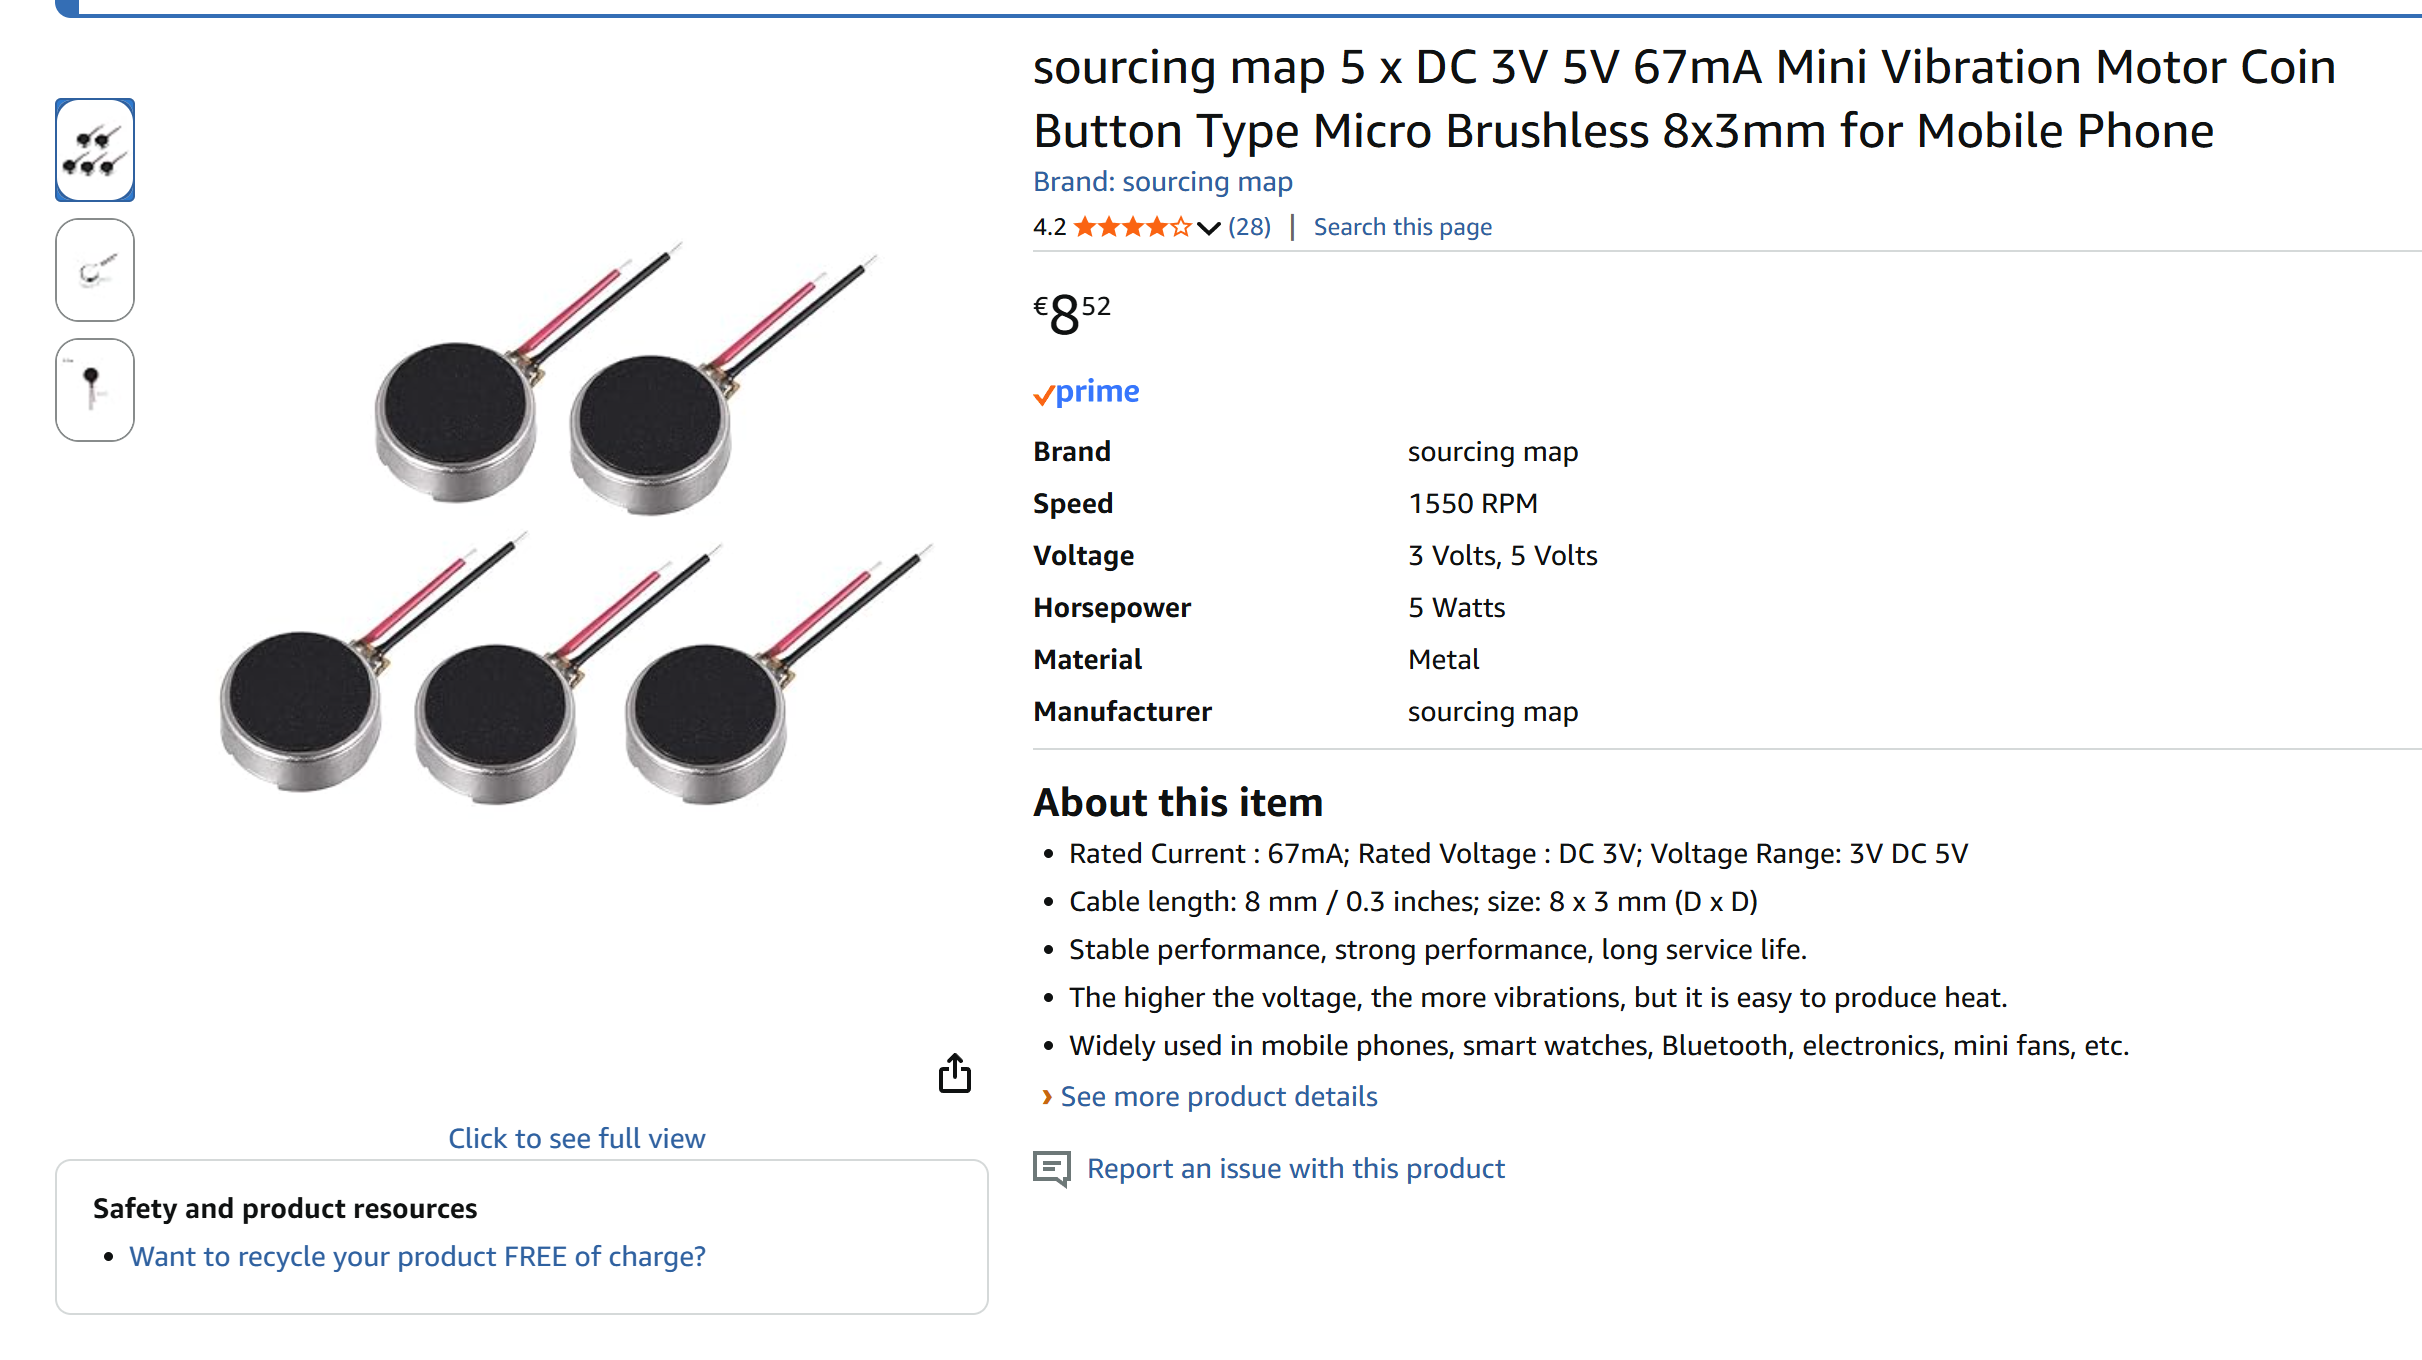
\includegraphics[width=\linewidth]{c3_haptic_motor.png}
    \caption{Supplier specification image of the coin vibration motor.}
    \label{fig:haptic_motor_spec}
\end{figure}

\chapter{Ethical Approval}\label{app:ethics}

The pilot field study was reviewed and approved under the project ``Daily Monitoring of Pelvic Rotation Using Wearable IMUs'' by the KU Leuven Privacy and Ethics platform (PRET), approval number \texttt{G-2025-10284-R2(MIN)}, dated 5 January 2026. The application was assessed for compliance with the General Data Protection Regulation (GDPR) by the data protection officer and reviewed for ethical standards by the Social and Societal Ethics Committee (SMEC); both gave a favourable decision. All participants gave informed consent before data collection and were free to stop or withdraw at any time.

\end{singlecolumnsection}


\backcover
\end{document}
